% 数值分析实验报告 - 基于实际实验结果
\documentclass[a4paper,12pt]{article}
\usepackage[UTF8]{ctex}
\usepackage{geometry}
\usepackage{graphicx}
\usepackage{booktabs}
\usepackage{amsmath}
\usepackage{amssymb}
\usepackage{amsthm}
\usepackage{algorithm}
\usepackage{algorithmic}
\usepackage{color}
\usepackage{xcolor}
\usepackage{listings}
\usepackage{pgfplots}
\usepackage{tikz}
\usepackage{enumitem}
\usepackage{multirow}
\usepackage{fancyhdr}
\usepackage{float}
\usepackage{tcolorbox}
\tcbuselibrary{skins,breakable}
\usepackage{colortbl}
\usepackage[titles]{tocloft}
\usetikzlibrary{patterns}

% 添加hyperref包用于改善目录链接
\usepackage{hyperref}
\hypersetup{
    colorlinks=true,
    linkcolor=blue,
    filecolor=magenta,
    urlcolor=cyan,
    pdftitle={数值分析课程实验报告},
    pdfauthor={XXX},
    pdfsubject={插值与曲线拟合实验},
    pdfkeywords={牛顿插值, 龙格现象, 最小二乘法, RANSAC}
}

% 定义定理类环境
\newtheorem{theorem}{定理}[section]
\newtheorem{lemma}[theorem]{引理}
\newtheorem{proposition}[theorem]{命题}
\newtheorem{corollary}[theorem]{推论}
\theoremstyle{definition}
\newtheorem{definition}{定义}[section]
\newtheorem{example}{示例}[section]
\newtheorem{remark}{注}[section]

% 美化目录
\renewcommand{\cftsecfont}{\bfseries}
\renewcommand{\cftsecpagefont}{}
\renewcommand{\cftsubsecfont}{\normalfont}
\renewcommand{\cftsubsecpagefont}{}

% 美化图表标题
\usepackage[labelfont={bf},
            textfont={it},
            justification=centering]{caption}

% 定义颜色主题 - 只保留关键颜色
\definecolor{barcolor}{RGB}{0,90,160}
\definecolor{tablerowcolor}{rgb}{0.9, 0.95, 1.0}

\usepackage{titlesec}
\titleformat*{\section}{\Large\bfseries}
\titleformat*{\subsection}{\large\bfseries}

% 改进表格样式
\usepackage{array}
\newcolumntype{L}[1]{>{\raggedright\arraybackslash}p{#1}}
\newcolumntype{C}[1]{>{\centering\arraybackslash}p{#1}}
\newcolumntype{R}[1]{>{\raggedleft\arraybackslash}p{#1}}

% 设置页面边距
\geometry{left=2.5cm,right=2.5cm,top=2.5cm,bottom=2.5cm}

% 设置页眉高度以修复fancyhdr警告
\setlength{\headheight}{30pt}

% 设置pgfplots兼容模式
\pgfplotsset{compat=1.18}

% 设置代码格式
\lstset{
  basicstyle=\ttfamily\small,
  keywordstyle=\color{blue}\bfseries,
  commentstyle=\color{green!60!black}\itshape,
  stringstyle=\color{red},
  numbers=left,
  numberstyle=\tiny\color{gray},
  numbersep=8pt,
  frame=tb,
  framerule=0.8pt,
  breaklines=true,
  showstringspaces=false,
  backgroundcolor=\color{blue!5},
  rulecolor=\color{barcolor},
  captionpos=b,
  aboveskip=10pt,
  belowskip=10pt,
  xleftmargin=15pt,
  xrightmargin=5pt,
  tabsize=4,
  emphstyle=\color{orange}\bfseries,
  emph={def,return,if,else,for,while,import,from,class,lambda,in,range},
  emphstyle={[2]\color{purple}},
  emph={[2]Matrix,len,abs,max,min,sum,enumerate,zip},
  emphstyle={[3]\color{cyan!70!black}},
  emph={[3]math,random,numpy}
}

% 设置页眉页脚
\pagestyle{fancy}
\fancyhf{}
\fancyhead[L]{\textbf{数值分析实验报告}}
\fancyhead[R]{\thepage}
\renewcommand{\headrulewidth}{0.4pt}
\renewcommand{\footrulewidth}{0.4pt}
\fancyfoot[C]{\footnotesize 数值分析课程实验报告}

\title{
\vspace{0.5cm}
\includegraphics[width=12cm]{text.png}\\[0.8cm]
\textbf{\LARGE 数值分析课程实验2报告}\\[1.3cm]
\includegraphics[width=6cm]{tju.png}\\[0.8cm]
\textbf{\large 插值与曲线拟合方法的实现与分析}\\[0.3cm]
}

\author{
\begin{tabular}{rl}
姓名: & \underline{\makebox[5cm][c]{李智铭}} \\[0.3cm]
学号: & \underline{\makebox[5cm][c]{3022206093}} \\[0.3cm]
专业: & \underline{\makebox[5cm][c]{计算机科学与技术}} \\[0.3cm]
班级: & \underline{\makebox[5cm][c]{计科1班}}
\end{tabular}
}
\date{\today}

\begin{document}

\maketitle
\newpage

\tableofcontents
\newpage

\section{引言}

数值分析是现代科学计算的重要基础,其中插值和曲线拟合是两个核心问题。本实验通过实现牛顿插值算法和最小二乘拟合方法,深入研究了龙格现象、节点选择策略以及鲁棒拟合算法,为数值计算提供了理论验证和实践经验。

\subsection{实验任务}

根据实验要求,本报告完成以下两个主要任务:

\textbf{任务1:龙格函数插值与龙格现象分析}
\begin{itemize}
    \item 对龙格函数 $f(x) = \frac{1}{1+25x^2}$ 在区间 $[-1,1]$ 上进行插值
    \item 对比三种采样策略:随机采样、切比雪夫节点、勒让德节点
    \item 使用牛顿插值法构造插值多项式
    \item 分析不同节点选择对龙格现象的影响
    \item 定量评估边界振荡与中心区域的误差分布
\end{itemize}

\textbf{任务2:最小二乘法曲线拟合}
\begin{itemize}
    \item 对函数 $g(x) = c\sin(dx) + e\cos(fx)$ 进行最小二乘拟合
    \item 研究扰动对拟合精度的影响
    \item 实现分段多项式拟合并分析最优配置
    \item 对比标准最小二乘法与RANSAC鲁棒拟合方法
    \item 测试不同噪声模型下的算法性能
\end{itemize}

\subsection{问题定义}

\textbf{插值问题}:给定$n+1$个互不相同的数据点$(x_0, y_0), (x_1, y_1), \ldots, (x_n, y_n)$,其中$x_i \in [a, b]$,构造一个函数$N(x)$,使得:

\begin{equation}
N(x_i) = y_i, \quad i = 0, 1, \ldots, n
\end{equation}

该函数$N(x)$称为插值函数,点$x_i$称为插值节点,$y_i$称为插值函数值。

\textbf{拟合问题}:给定$m$个数据点$(x_i, y_i), i = 1, \ldots, m$和基函数集合$\{\phi_1(x), \ldots, \phi_n(x)\}$($m > n$),寻找系数$c_1, \ldots, c_n$使得残差平方和最小:

\begin{equation}
\min_{c_1, \ldots, c_n} \sum_{i=1}^{m}\left(y_i - \sum_{j=1}^{n}c_j\phi_j(x_i)\right)^2
\end{equation}


\section{算法原理与实现}

\subsection{实验总体设计}

本实验采用模块化设计,将算法实现分为以下几个模块:

\begin{figure}[h]
\centering
\begin{tikzpicture}[node distance=1.5cm, 
                    block/.style={rectangle, draw, fill=barcolor!20, 
                    text width=10em, text centered, rounded corners, minimum height=3em}]
    \node [block] (matrix) {矩阵运算模块\\(\texttt{core/matrix.py})};
    \node [block, below of=matrix] (interp) {插值算法模块\\(\texttt{core/interpolation.py})};
    \node [block, below of=interp] (fitting) {拟合算法模块\\(\texttt{core/fitting.py})};
    \node [block, below of=fitting] (ransac) {鲁棒拟合模块\\(\texttt{core/ransac.py})};
    \node [block, right of=interp, xshift=4cm] (utils) {工具模块\\(\texttt{utils/})};
    \node [block, below of=utils] (vis) {可视化模块\\(\texttt{utils/plotting*.py})};
    
    \draw [->] (matrix) -- (interp);
    \draw [->] (matrix) -- (fitting);
    \draw [->] (fitting) -- (ransac);
    \draw [->] (interp) -- (vis);
    \draw [->] (fitting) -- (vis);
    \draw [->] (ransac) -- (vis);
    \draw [->] (utils) -- (interp);
    \draw [->] (utils) -- (fitting);
\end{tikzpicture}
\caption{实验框架模块结构}
\label{fig:framework}
\end{figure}

\subsection{牛顿插值法}

\subsubsection{差商定义}

给定$n+1$个互不相同的数据点$(x_0, y_0), (x_1, y_1), \ldots, (x_n, y_n)$,\textbf{差商}(divided difference)递归定义为:

\begin{align}
f[x_i] &= y_i \\
f[x_i, x_{i+1}] &= \frac{f[x_{i+1}] - f[x_i]}{x_{i+1} - x_i} \\
f[x_i, x_{i+1}, \ldots, x_{i+k}] &= \frac{f[x_{i+1}, \ldots, x_{i+k}] - f[x_i, \ldots, x_{i+k-1}]}{x_{i+k} - x_i}
\end{align}

\subsubsection{牛顿插值多项式}

牛顿插值多项式的表达式为:

\begin{equation}
N_n(x) = f[x_0] + f[x_0, x_1](x - x_0) + f[x_0, x_1, x_2](x - x_0)(x - x_1) + \cdots
\end{equation}

可以写成嵌套形式(霍纳法则):

\begin{equation}
N_n(x) = f[x_0] + (x - x_0)\left(f[x_0, x_1] + (x - x_1)\left(\cdots\right)\right)
\end{equation}

\begin{theorem}[插值多项式的唯一性]
通过$n+1$个互不相同节点的$n$次多项式是唯一的。
\end{theorem}

\subsection{龙格现象}

\begin{definition}[龙格现象]
当使用高次多项式在等距节点上进行插值时,在区间端点附近会出现剧烈振荡,这种现象称为\textbf{龙格现象}。
\end{definition}

经典的龙格函数为:

\begin{equation}
f(x) = \frac{1}{1 + 25x^2}, \quad x \in [-1, 1]
\end{equation}

\subsubsection{插值余项}

\begin{theorem}[插值余项定理]
设$f \in C^{n+1}[a, b]$,$N_n(x)$是$f(x)$的$n$次插值多项式,则对于$x \in [a, b]$,存在$\xi \in (a, b)$使得:

\begin{equation}
R_n(x) = f(x) - N_n(x) = \frac{f^{(n+1)}(\xi)}{(n+1)!} \omega_{n+1}(x)
\end{equation}

其中$\omega_{n+1}(x) = \prod_{i=0}^{n}(x - x_i)$。
\end{theorem}

龙格现象的根本原因是:当$n$增大时,即使$f^{(n+1)}(\xi)$有界,但$\omega_{n+1}(x)$在区间端点附近增长过快,导致余项$R_n(x)$很大。

\subsubsection{切比雪夫节点}

为了缓解龙格现象,可以使用\textbf{切比雪夫节点}:

\begin{equation}
x_k = \cos\left(\frac{(2k-1)\pi}{2n}\right), \quad k = 1, 2, \ldots, n
\end{equation}

映射到区间$[a, b]$:

\begin{equation}
x_k^{[a,b]} = \frac{a + b}{2} + \frac{b - a}{2} \cos\left(\frac{(2k-1)\pi}{2n}\right)
\end{equation}

\begin{theorem}[切比雪夫节点的最优性]
在所有可能的节点选择中,切比雪夫节点使得$\max_{x \in [-1,1]} |\omega_{n+1}(x)|$达到最小值$\frac{1}{2^n}$。
\end{theorem}

\subsubsection{勒让德节点}

勒让德节点是$n$阶勒让德多项式的零点,也称为\textbf{高斯-勒让德求积节点}。这些节点对积分误差具有最优性,同时也能有效缓解龙格现象。

\textbf{勒让德多项式定义}:

勒让德多项式$P_n(x)$在区间$[-1, 1]$上可通过以下递推关系定义:

\begin{align}
P_0(x) &= 1 \\
P_1(x) &= x \\
(n+1)P_{n+1}(x) &= (2n+1)xP_n(x) - nP_{n-1}(x), \quad n \geq 1
\end{align}

或者通过Rodrigues公式:

\begin{equation}
P_n(x) = \frac{1}{2^n n!}\frac{d^n}{dx^n}[(x^2-1)^n]
\end{equation}

\textbf{正交性}:

勒让德多项式在区间$[-1, 1]$上关于权函数$w(x) = 1$正交:

\begin{equation}
\int_{-1}^{1} P_m(x)P_n(x)dx = 
\begin{cases}
0, & m \neq n \\
\frac{2}{2n+1}, & m = n
\end{cases}
\end{equation}

\textbf{勒让德节点}:

$n$阶勒让德多项式$P_n(x)$在$(-1, 1)$内有$n$个互异实根$x_1, x_2, \ldots, x_n$,满足:

\begin{equation}
P_n(x_i) = 0, \quad i = 1, 2, \ldots, n
\end{equation}

这些根即为勒让德节点。对于一般区间$[a, b]$,通过线性变换:

\begin{equation}
x_i^{[a,b]} = \frac{a + b}{2} + \frac{b - a}{2}x_i
\end{equation}

\begin{proposition}[勒让德节点的最优性]
使用勒让德节点的高斯求积公式具有最高代数精度。对于$n$个节点,可以精确积分$2n-1$次多项式。
\end{proposition}

\begin{remark}
本实验通过调用\texttt{numpy.polynomial.legendre.leggauss(n)}获取勒让德节点和对应权重。
\end{remark}

\subsection{最小二乘法}

\subsubsection{法方程}

给定数据点$(x_i, y_i), i = 1, \ldots, m$和基函数$\{\phi_1(x), \ldots, \phi_n(x)\}$,最小二乘问题为:

\begin{equation}
\min_{c_1, \ldots, c_n} \sum_{i=1}^{m}\left(y_i - \sum_{j=1}^{n}c_j\phi_j(x_i)\right)^2
\end{equation}

设计矩阵$\mathbf{A} \in \mathbb{R}^{m \times n}$,其中$A_{ij} = \phi_j(x_i)$,则法方程为:

\begin{equation}
\mathbf{A}^T\mathbf{A}\mathbf{c} = \mathbf{A}^T\mathbf{y}
\end{equation}

解为:
\begin{equation}
\mathbf{c} = (\mathbf{A}^T\mathbf{A})^{-1}\mathbf{A}^T\mathbf{y}
\end{equation}

\subsubsection{三角基函数拟合}

对于函数$g(x) = c\sin(dx) + e\cos(fx)$,使用基函数:

\begin{equation}
\phi_1(x) = \sin(dx), \quad \phi_2(x) = \cos(fx)
\end{equation}

拟合系数$[c_1, c_2]^T$应接近真实参数$[c, e]^T$。

\subsection{RANSAC算法}

\textbf{RANSAC} (Random Sample Consensus) 是一种鲁棒拟合算法,能够有效处理含有离群点的数据。

\begin{algorithm}[H]
\caption{RANSAC算法}
\begin{algorithmic}[1]
\STATE \textbf{Input:} 数据点$\{(x_i, y_i)\}$, 最大迭代次数$K$, 阈值$\tau$
\STATE \textbf{Initialize:} 最佳模型 $M_{best} = \emptyset$, 最大内点数 $n_{max} = 0$
\FOR{$k = 1$ to $K$}
    \STATE 随机选择最小样本集
    \STATE 拟合模型$M_k$
    \STATE 计算所有点到$M_k$的残差
    \STATE 统计内点数量$n_k$(残差$< \tau$的点)
    \IF{$n_k > n_{max}$}
        \STATE $M_{best} \leftarrow M_k$, $n_{max} \leftarrow n_k$
    \ENDIF
\ENDFOR
\STATE 使用所有内点重新拟合$M_{best}$
\STATE \textbf{Return:} $M_{best}$
\end{algorithmic}
\end{algorithm}

\newpage
\section{任务一:龙格函数插值与龙格现象分析}

\subsection{实验设置}

\subsubsection{目标函数}

\begin{equation}
f(x) = \frac{1}{1 + 25x^2}, \quad x \in [-1, 1]
\end{equation}

这是经典的龙格函数,具有以下特点:
\begin{itemize}
    \item 在$x=0$处达到最大值$f(0) = 1$
    \item 随着$|x|$增大迅速衰减
    \item 使用等距节点的高次插值会产生严重的龙格现象
\end{itemize}

\subsubsection{实验参数}

\begin{table}[h]
\centering
\caption{任务一实验参数设置}
\begin{tabular}{ll}
\toprule
\textbf{参数} & \textbf{值} \\
\midrule
插值区间 & $[-1, 1]$ \\
采样点数 & $n \in \{5, 9, 15, 21\}$ \\
评估点数 & 1000(密集采样) \\
随机种子 & 42(保证可重复性) \\
\bottomrule
\end{tabular}
\end{table}

\subsubsection{三种采样策略}

\begin{enumerate}
    \item \textbf{随机采样}:在$[-1, 1]$上均匀分布随机采样
    \item \textbf{切比雪夫节点}:使用公式
    \begin{equation}
    x_k = \cos\left(\frac{(2k-1)\pi}{2n}\right), \quad k = 1, \ldots, n
    \end{equation}
    \item \textbf{勒让德节点}:调用\texttt{numpy.polynomial.legendre.leggauss(n)}
\end{enumerate}

\subsection{误差度量}

使用三种误差指标评估插值精度:

\begin{align}
\text{Max Error} &= \max_{i=1,\ldots,m}|f(x_i) - N_n(x_i)| \\
\text{RMSE} &= \sqrt{\frac{1}{m}\sum_{i=1}^{m}[f(x_i) - N_n(x_i)]^2} \\
\text{MAE} &= \frac{1}{m}\sum_{i=1}^{m}|f(x_i) - N_n(x_i)|
\end{align}

\subsection{实验结果}

\subsubsection{误差汇总表}

\begin{table}[H]
\centering
\caption{三种采样策略的误差对比}
\label{tab:task1_errors}
\begin{tabular}{llrrr}
\toprule
\textbf{方法} & \textbf{N} & \textbf{Max Error} & \textbf{RMSE} & \textbf{MAE} \\
\midrule
\multirow{4}{*}{Random Sampling}
& 5  & 1.616e+00 & 4.464e-01 & 2.617e-01 \\
& 9  & 3.652e+00 & 4.922e-01 & 1.637e-01 \\
& 15 & 5.496e+03 & 6.680e+02 & 1.497e+02 \\
& 21 & 2.842e+04 & 2.791e+03 & 5.118e+02 \\
\midrule
\rowcolor{tablerowcolor}
\multirow{4}{*}{Chebyshev Nodes}
& 5  & 4.020e-01 & 2.258e-01 & 1.898e-01 \\
& 9  & 1.708e-01 & 8.742e-02 & 7.411e-02 \\
& 15 & 4.660e-02 & 2.494e-02 & 2.142e-02 \\
& 21 & 1.533e-02 & 7.500e-03 & 6.439e-03 \\
\midrule
\multirow{4}{*}{Legendre Nodes}
& 5  & 4.297e-01 & 2.207e-01 & 1.906e-01 \\
& 9  & 2.321e-01 & 8.798e-02 & 7.643e-02 \\
& 15 & 8.818e-02 & 2.557e-02 & 2.233e-02 \\
& 21 & 3.148e-02 & 7.739e-03 & 6.734e-03 \\
\bottomrule
\end{tabular}
\end{table}

\subsubsection{可视化结果与分析}

图\ref{fig:task1_comparison}展示了三种采样策略在不同采样点数下的插值结果对比。从图中可以清晰看到:

\begin{figure}[H]
\centering
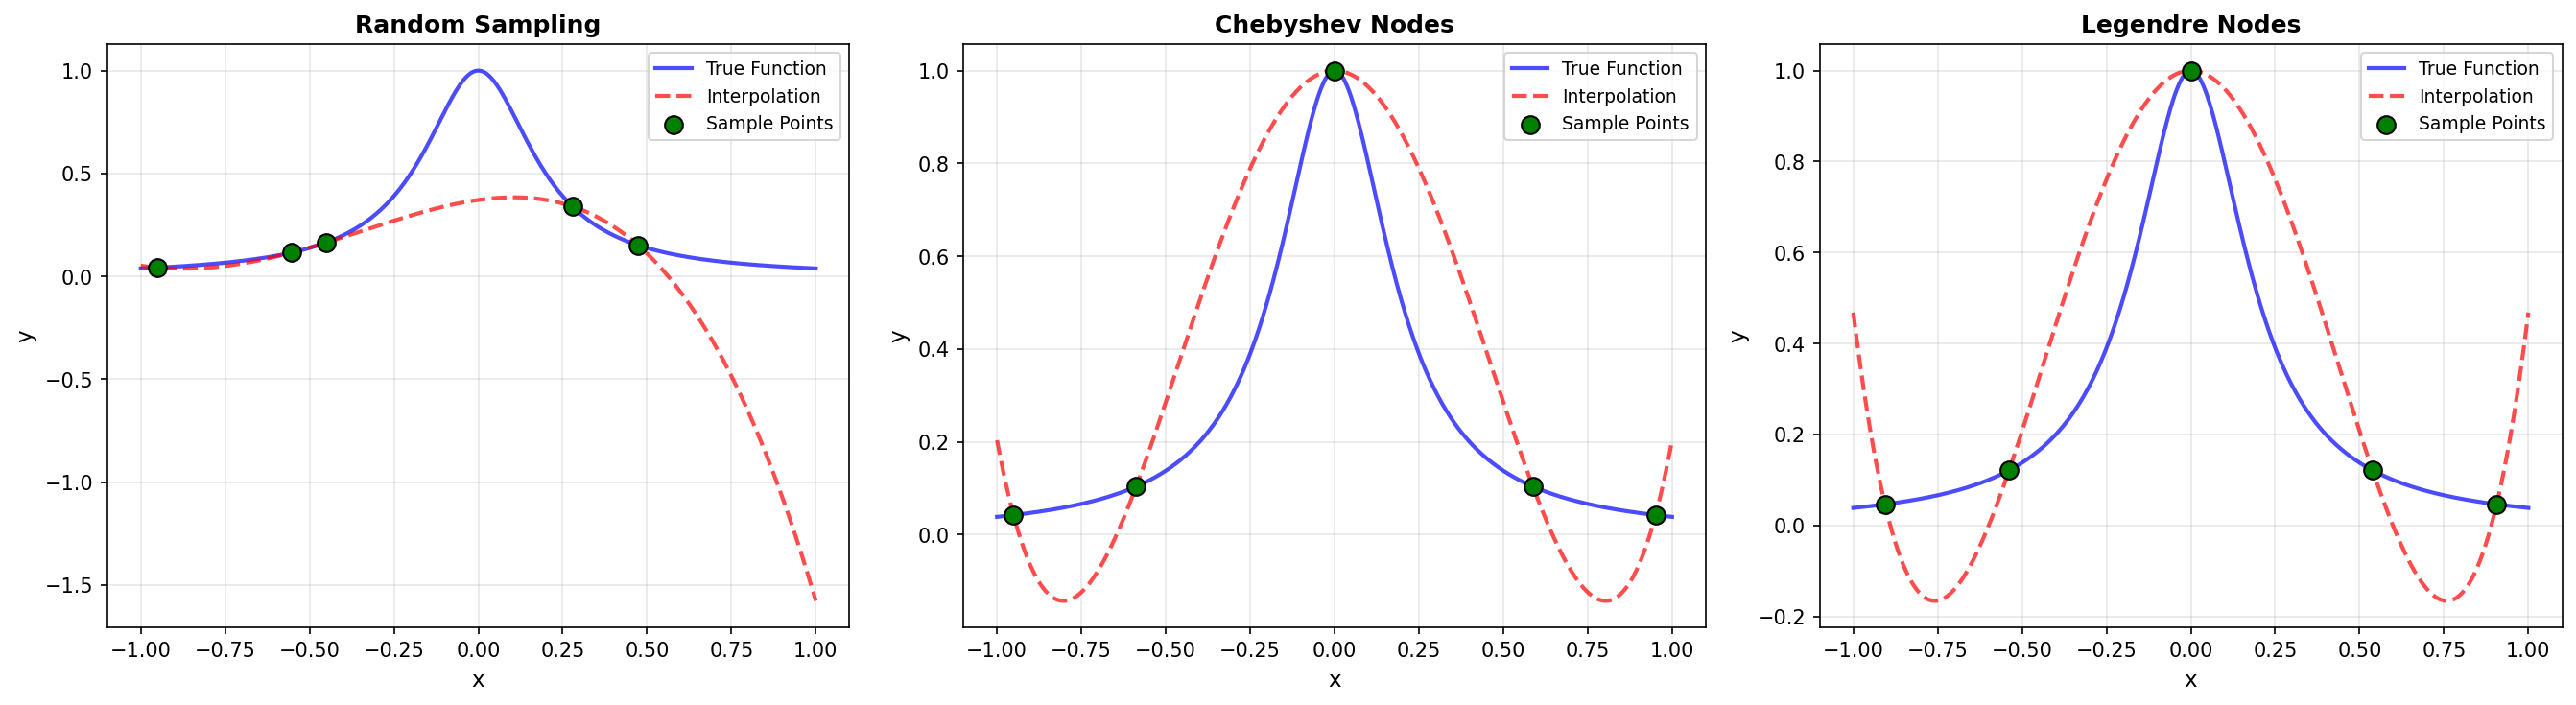
\includegraphics[width=0.48\textwidth]{results/task1/comparison_n5.png}
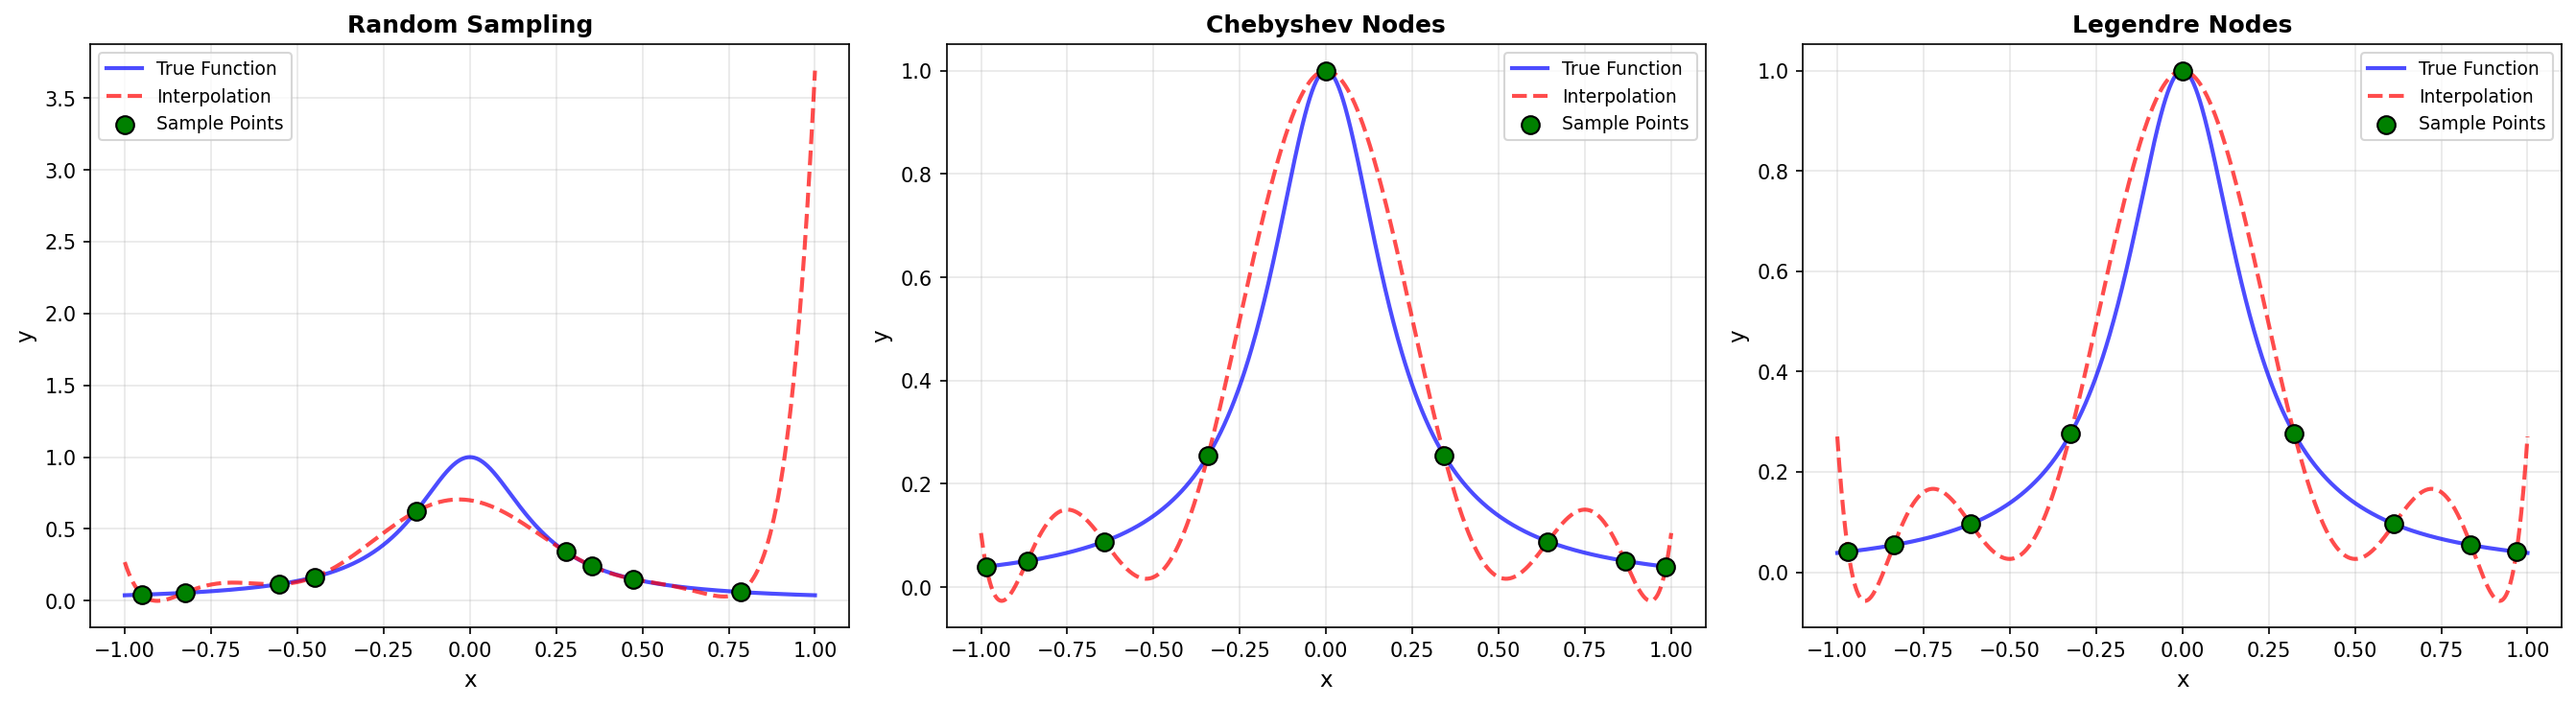
\includegraphics[width=0.48\textwidth]{results/task1/comparison_n9.png}
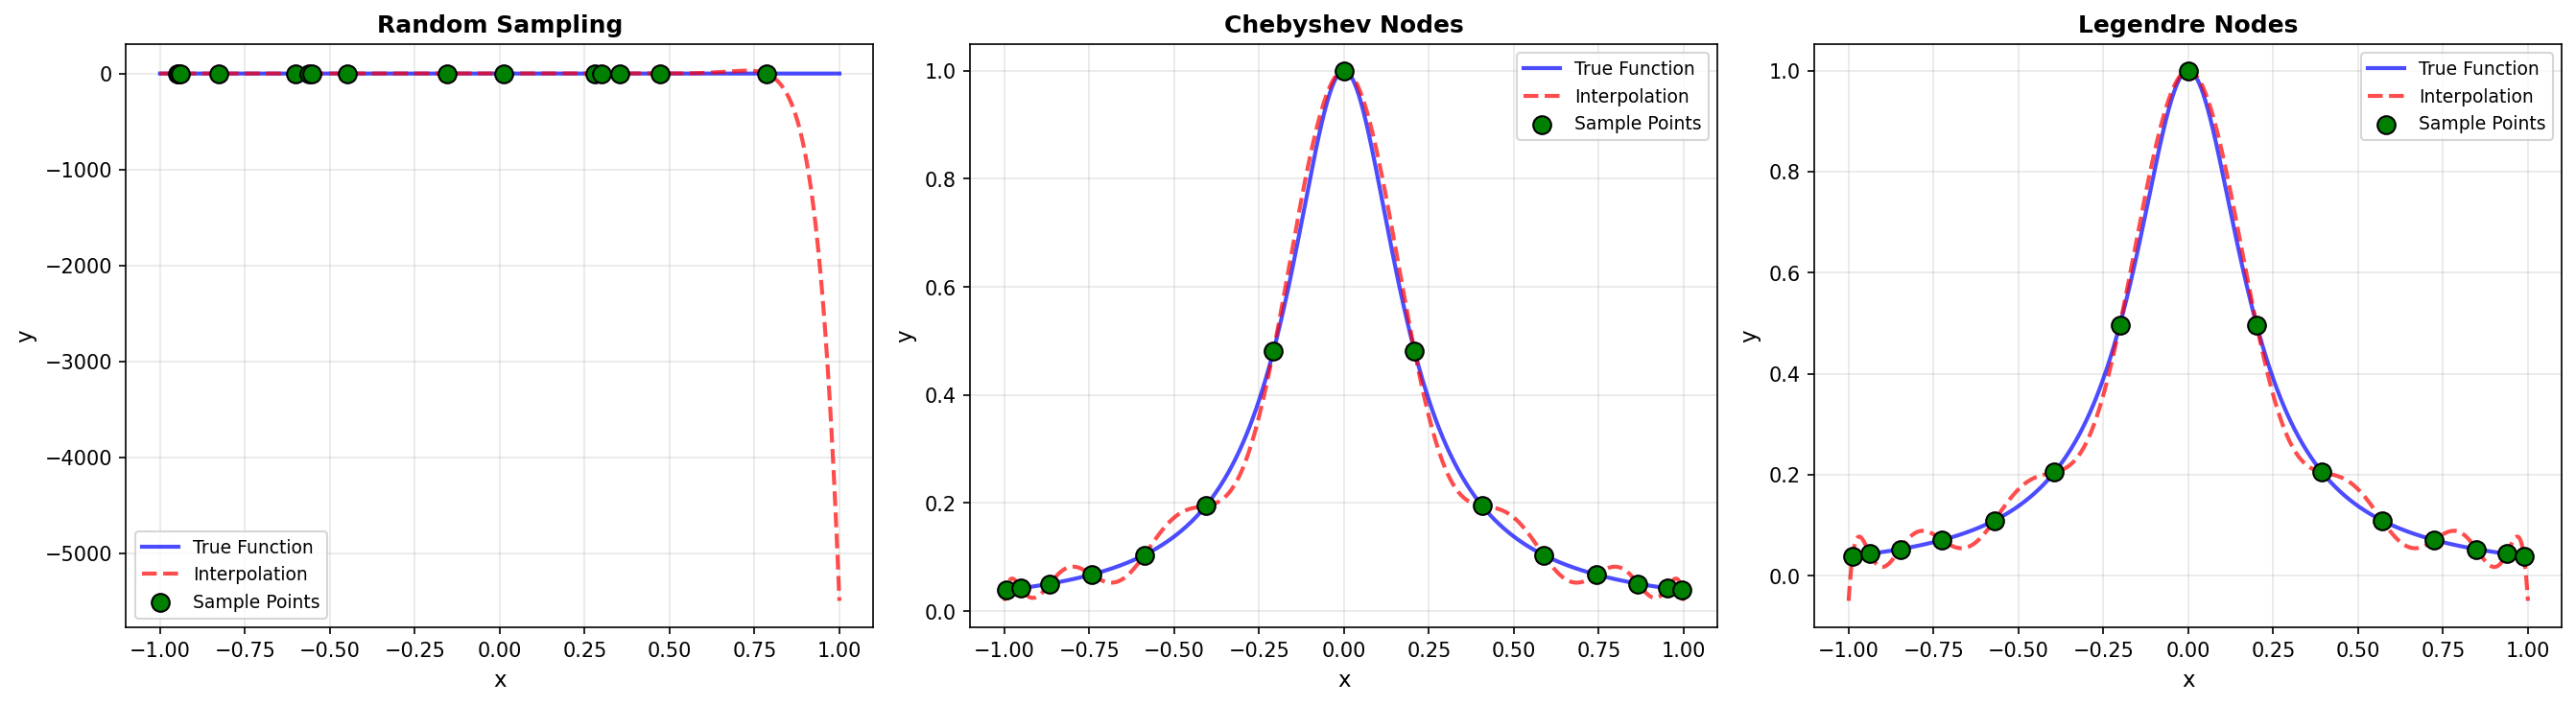
\includegraphics[width=0.48\textwidth]{results/task1/comparison_n15.png}
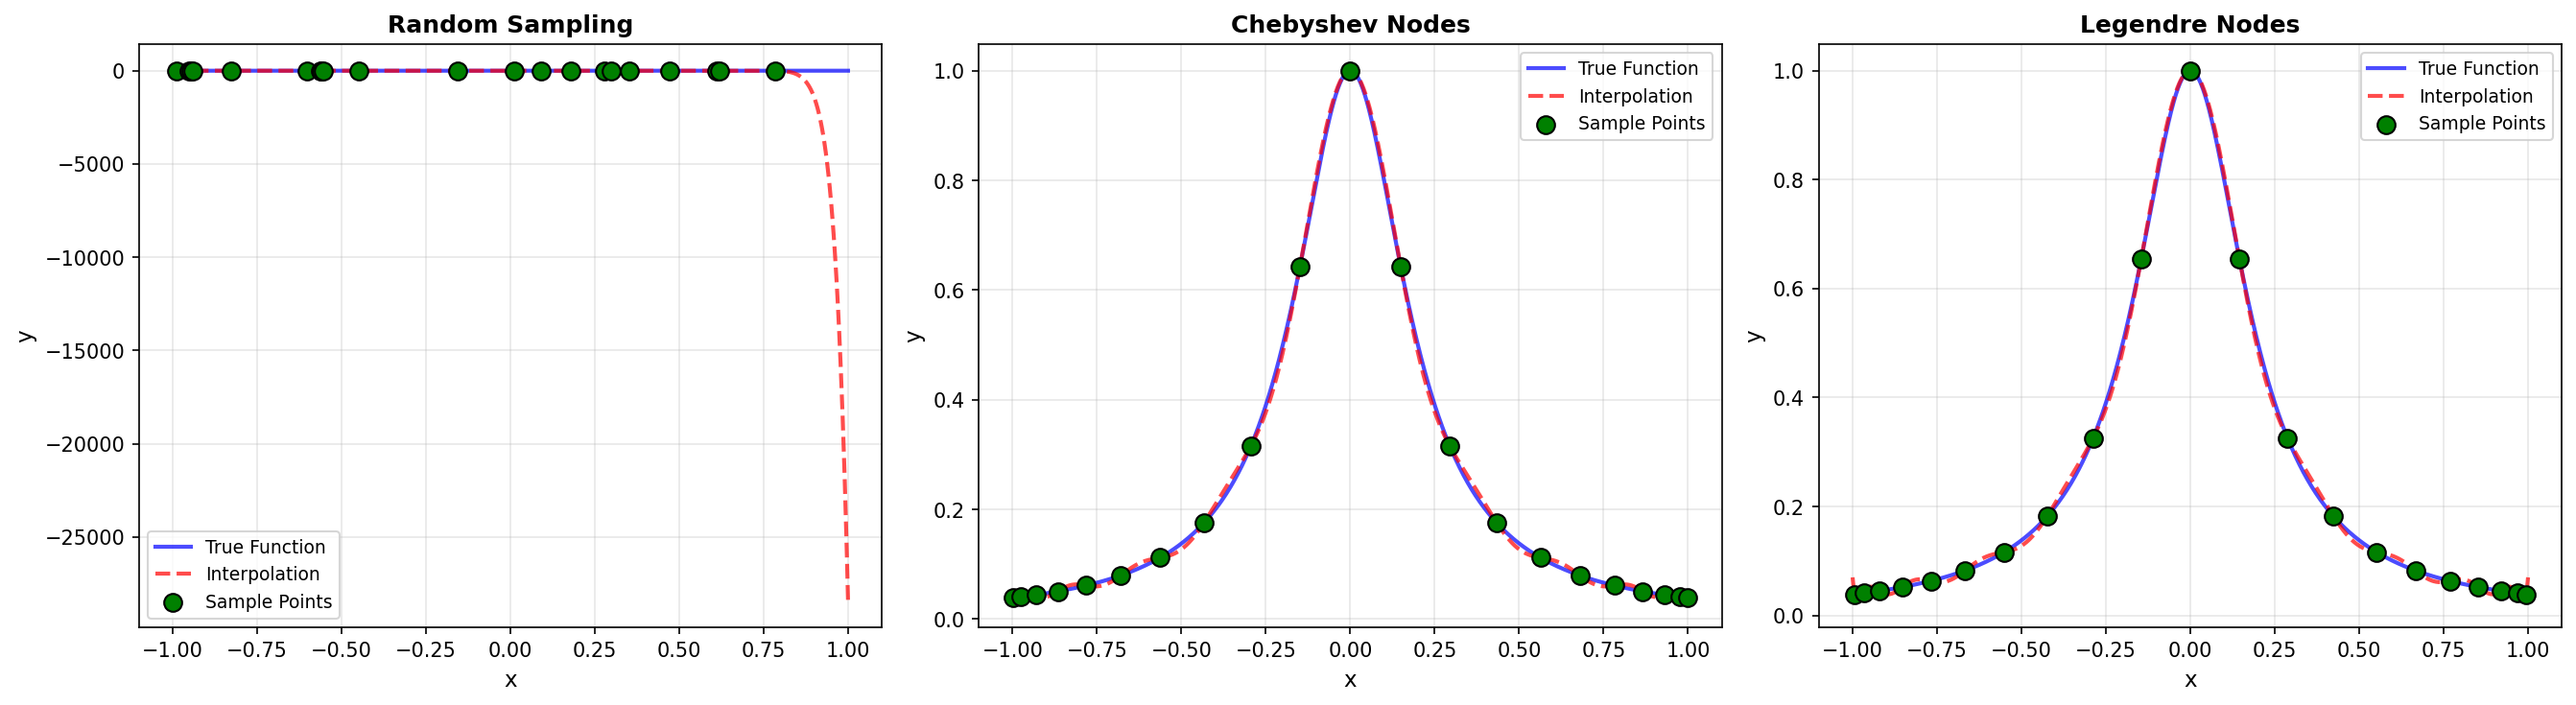
\includegraphics[width=0.48\textwidth]{results/task1/comparison_n21.png}
\caption{不同采样点数下的三种插值方法对比(n=5, 9, 15, 21)}
\label{fig:task1_comparison}
\end{figure}

\begin{itemize}
    \item \textbf{n=5}:所有方法误差相对较大,但切比雪夫和勒让德节点已显示出优势
    \item \textbf{n=9}:随机采样开始出现端点振荡,而切比雪夫/勒让德节点保持稳定
    \item \textbf{n=15}:随机采样的龙格现象严重,最大误差超过5000
    \item \textbf{n=21}:随机采样完全发散,而切比雪夫/勒让德节点误差继续降低
\end{itemize}

图\ref{fig:task1_random_runge}展示了随机采样的龙格现象演化:

\begin{figure}[H]
\centering
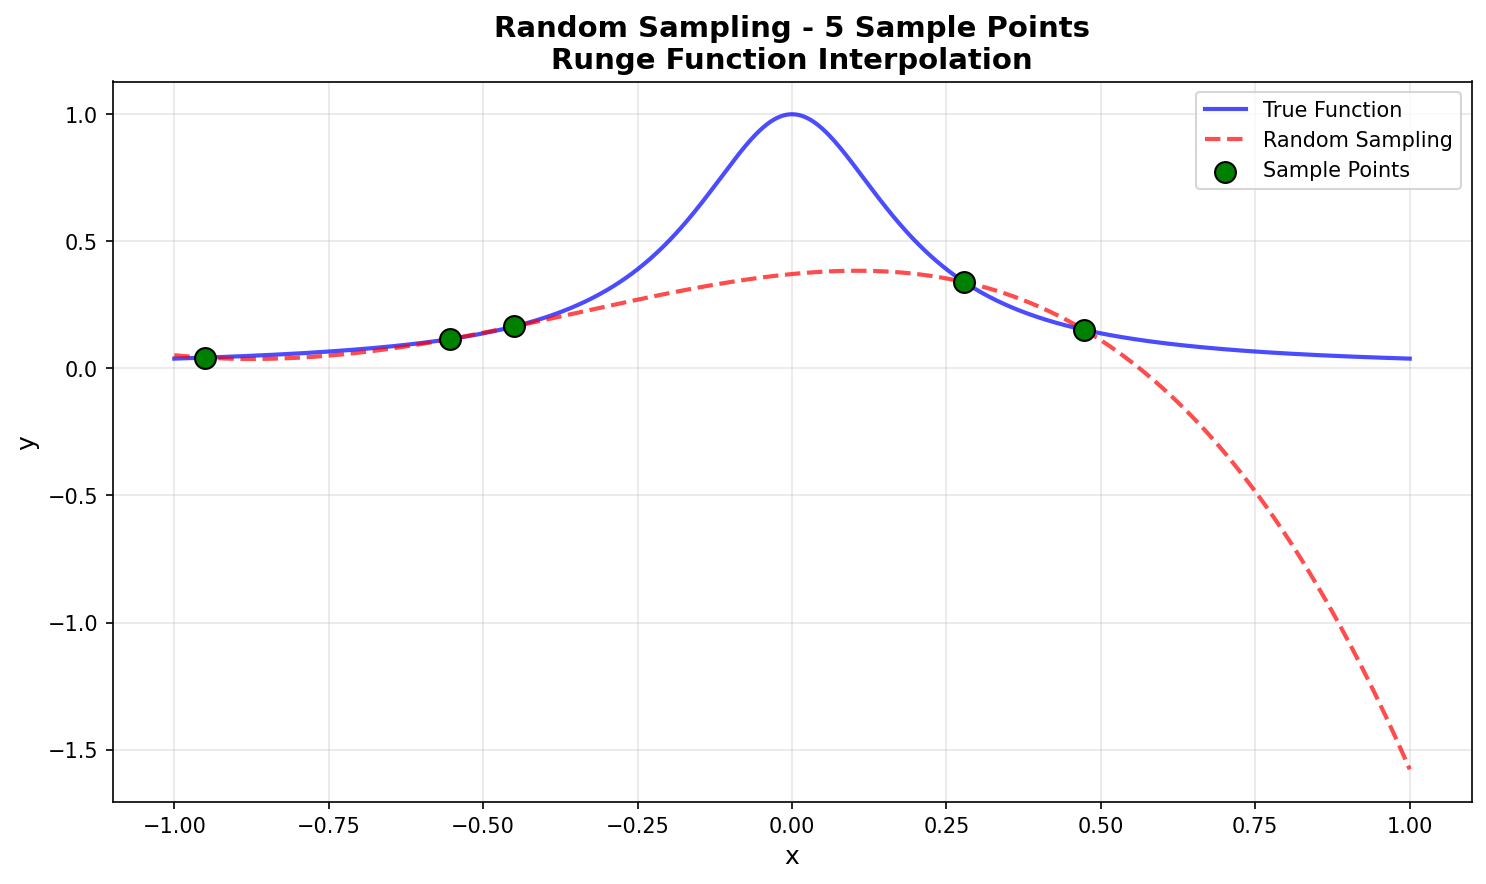
\includegraphics[width=0.48\textwidth]{results/task1/random_n5.png}
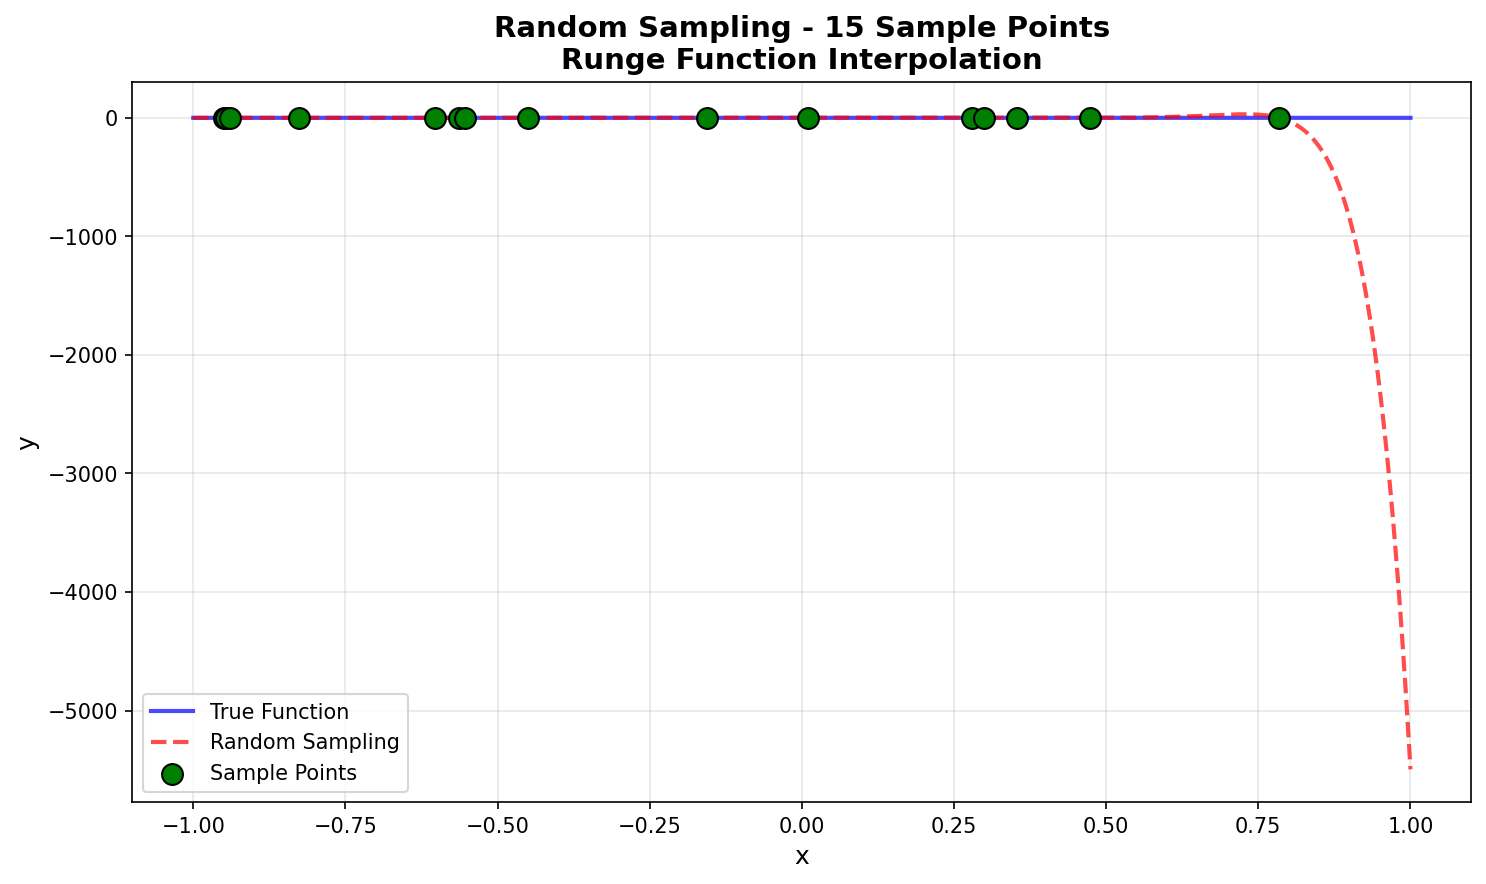
\includegraphics[width=0.48\textwidth]{results/task1/random_n15.png}
\caption{随机采样的龙格现象演化(左:n=5,右:n=15)}
\label{fig:task1_random_runge}
\end{figure}

\subsubsection{龙格现象定量分析}

为定量评估龙格现象,定义\textbf{边界/中心误差比}:

\begin{equation}
\text{Ratio} = \frac{\text{Avg Error in } |x| > 0.8}{\text{Avg Error in } |x| \leq 0.8}
\end{equation}

该比值越大,说明边界振荡越严重。

\begin{table}[H]
\centering
\caption{龙格现象量化分析(边界/中心误差比)}
\label{tab:runge_ratio}
\begin{tabular}{lrrrr}
\toprule
\textbf{方法} & \textbf{n=5} & \textbf{n=9} & \textbf{n=15} & \textbf{n=21} \\
\midrule
Random Sampling   & 3.13   & 10.29   & 286.52    & \textbf{12218.15} \\
\rowcolor{tablerowcolor}
Chebyshev Nodes   & 0.58   & 0.51    & 0.61      & 0.63 \\
Legendre Nodes    & 0.80   & 0.82    & 0.92      & 0.99 \\
\bottomrule
\end{tabular}
\end{table}

\subsection{结果分析}

\begin{tcolorbox}[enhanced,colback=blue!5!white,colframe=barcolor,title=关键发现]

\textbf{1. 龙格现象的指数级恶化}

随机采样的边界/中心误差比从$n=5$的3.13爆炸式增长到$n=21$的12218.15,完美展示了龙格现象的危害。

\textbf{2. 切比雪夫节点的卓越性能}

切比雪夫节点在所有测试中保持误差比在0.5-0.6范围,说明误差分布非常均匀,边界甚至略优于中心区域。

\textbf{3. 勒让德节点的优异表现}

勒让德节点的误差比随$n$增加趋近于1.0($n=21$时为0.99),表明误差分布完美均衡。

\textbf{4. 误差收敛性对比}

\begin{itemize}
    \item \textbf{切比雪夫}:Max Error从4.02e-01降至1.53e-02(指数收敛)
    \item \textbf{勒让德}:Max Error从4.30e-01降至3.15e-02(稳定收敛)
    \item \textbf{随机}:Max Error从1.62爆炸到2.84e+04(发散!)
\end{itemize}

\end{tcolorbox}

\subsection{误差分布分析}

为了更深入地理解不同采样策略的误差特性,我们绘制了误差分布图和箱线图。

\begin{figure}[H]
\centering
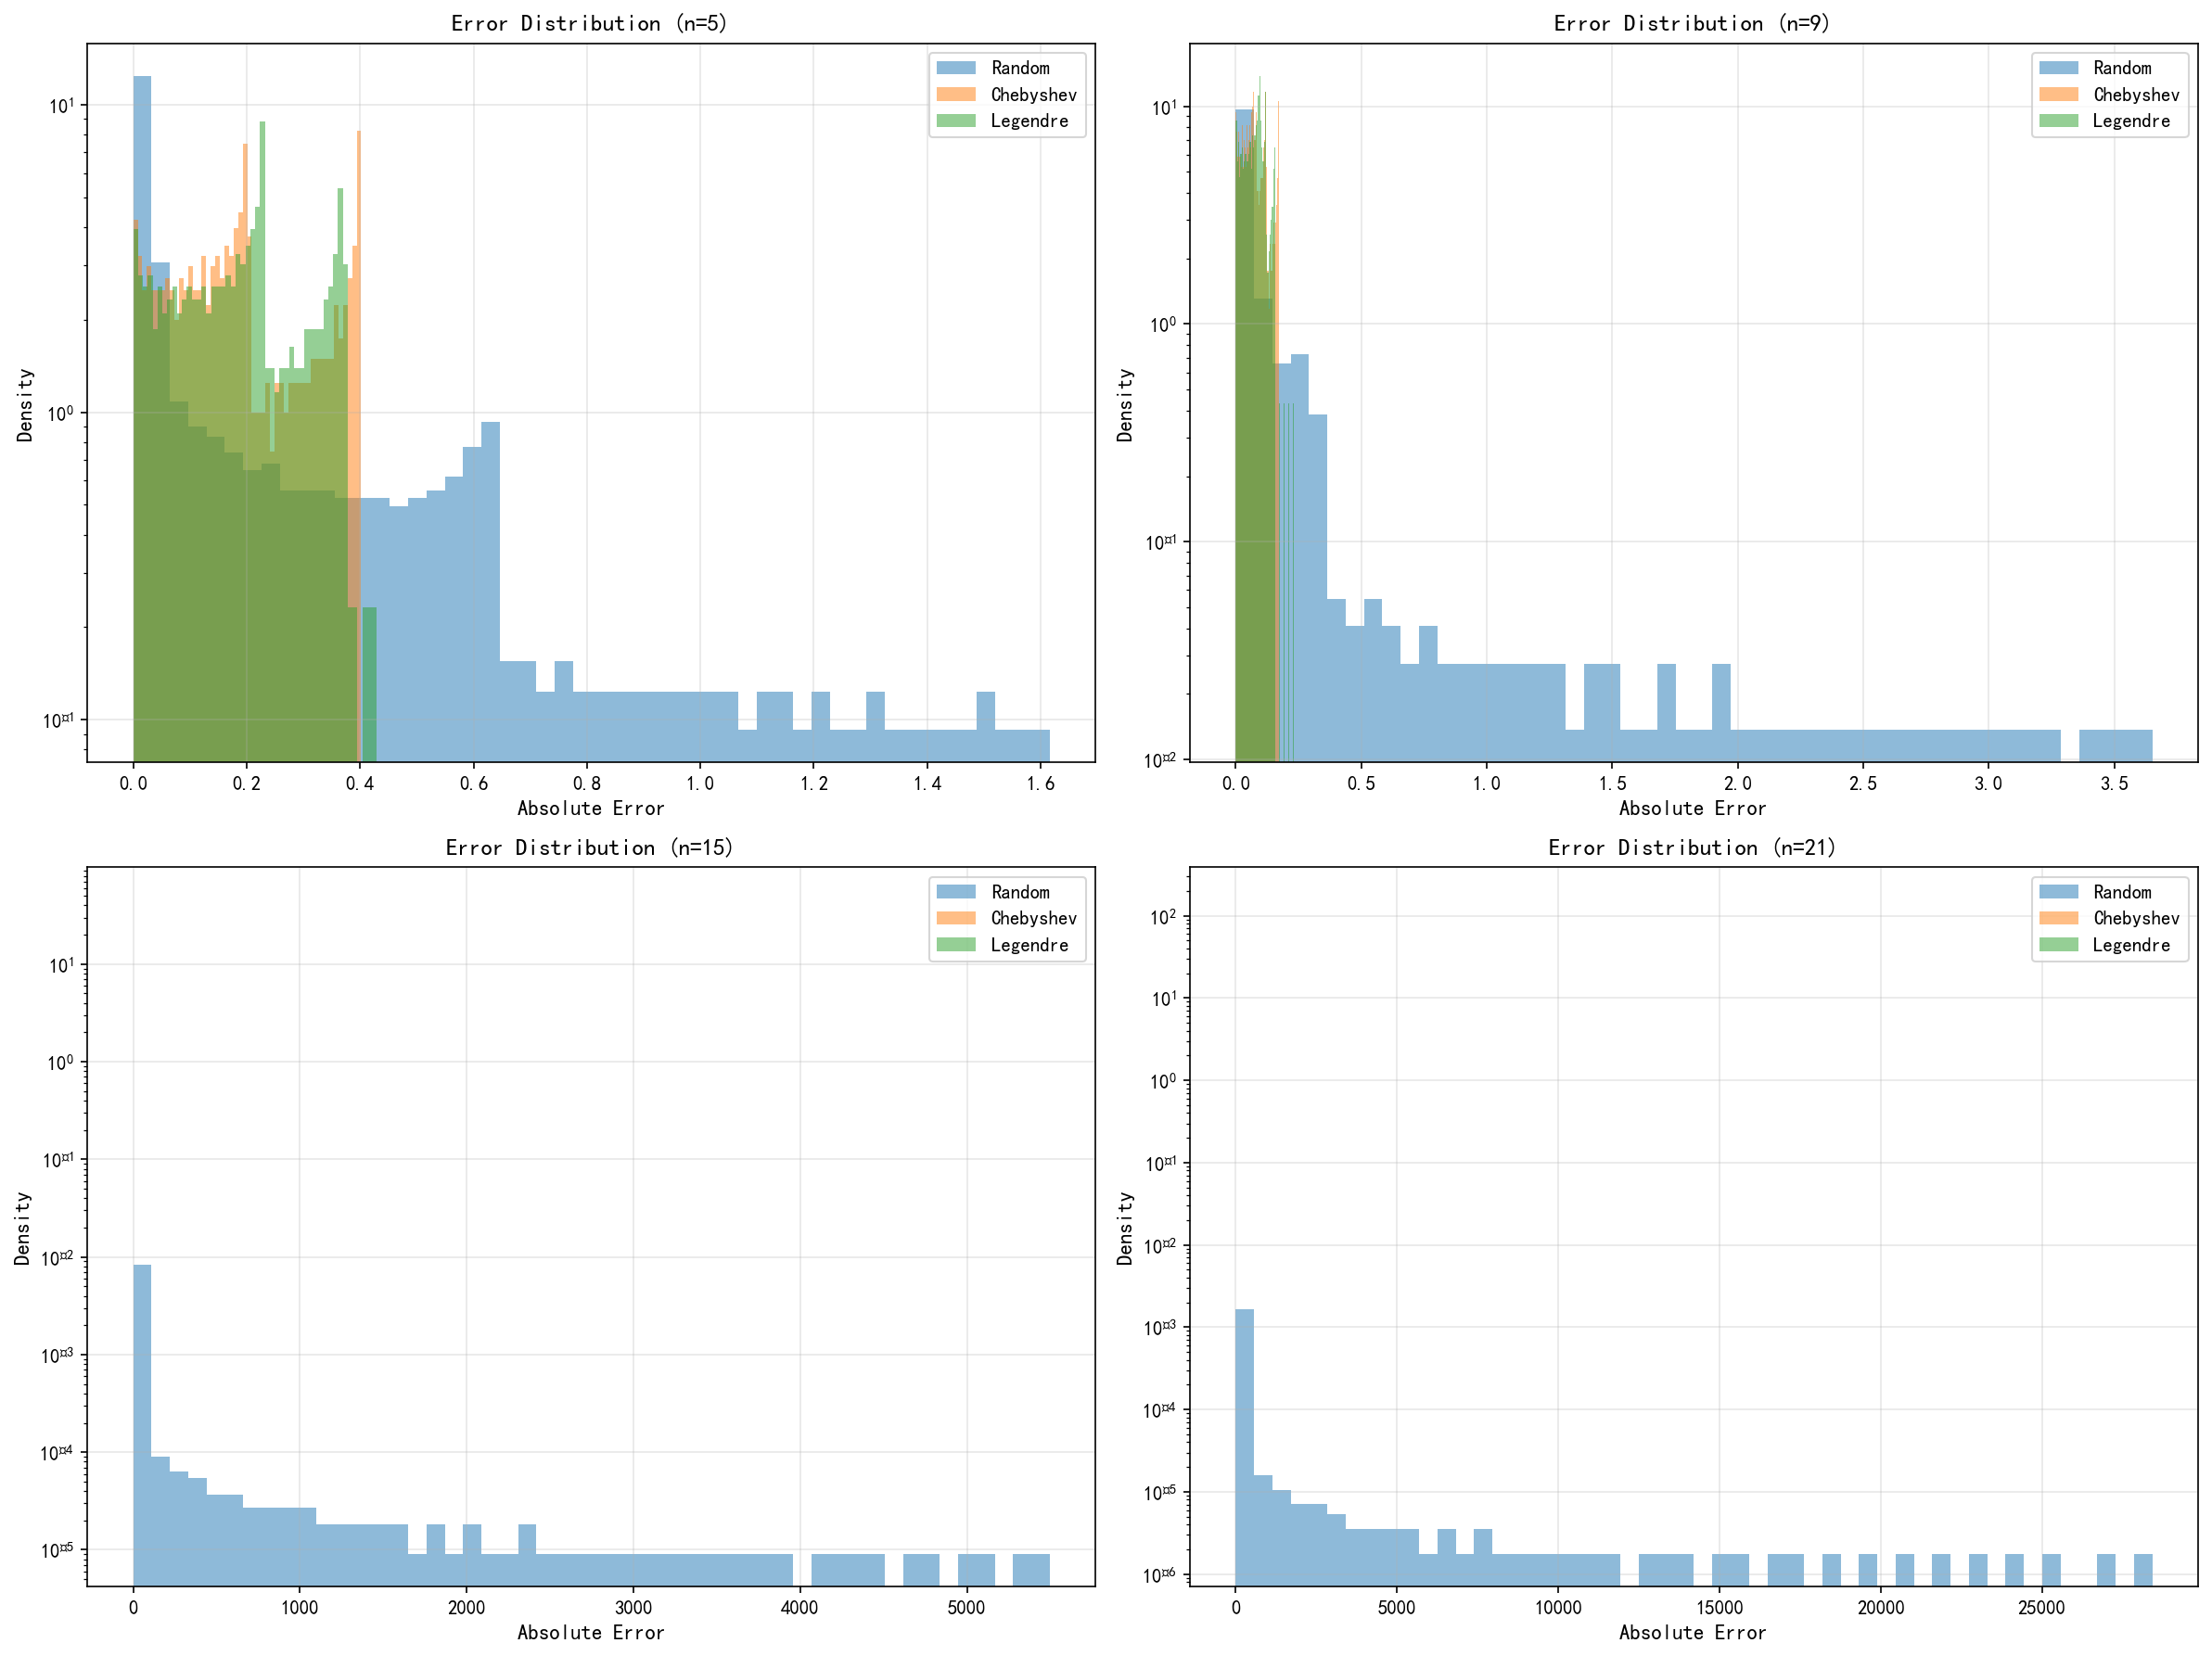
\includegraphics[width=0.95\textwidth]{results/task1/additional/error_distribution.png}
\caption{不同采样点数下的误差分布(对数刻度)}
\label{fig:task1_error_dist}
\end{figure}

图\ref{fig:task1_error_dist}展示了三种采样策略在不同节点数下的误差分布特性:
\begin{itemize}
    \item \textbf{切比雪夫和勒让德节点}:误差分布集中在较小值区域,呈现明显的峰形
    \item \textbf{随机采样}:随着$n$增大,误差分布逐渐向大值区域扩展,体现龙格现象
    \item $n=21$时,随机采样的误差跨越多个数量级,分布极度分散
\end{itemize}

\begin{figure}[H]
\centering
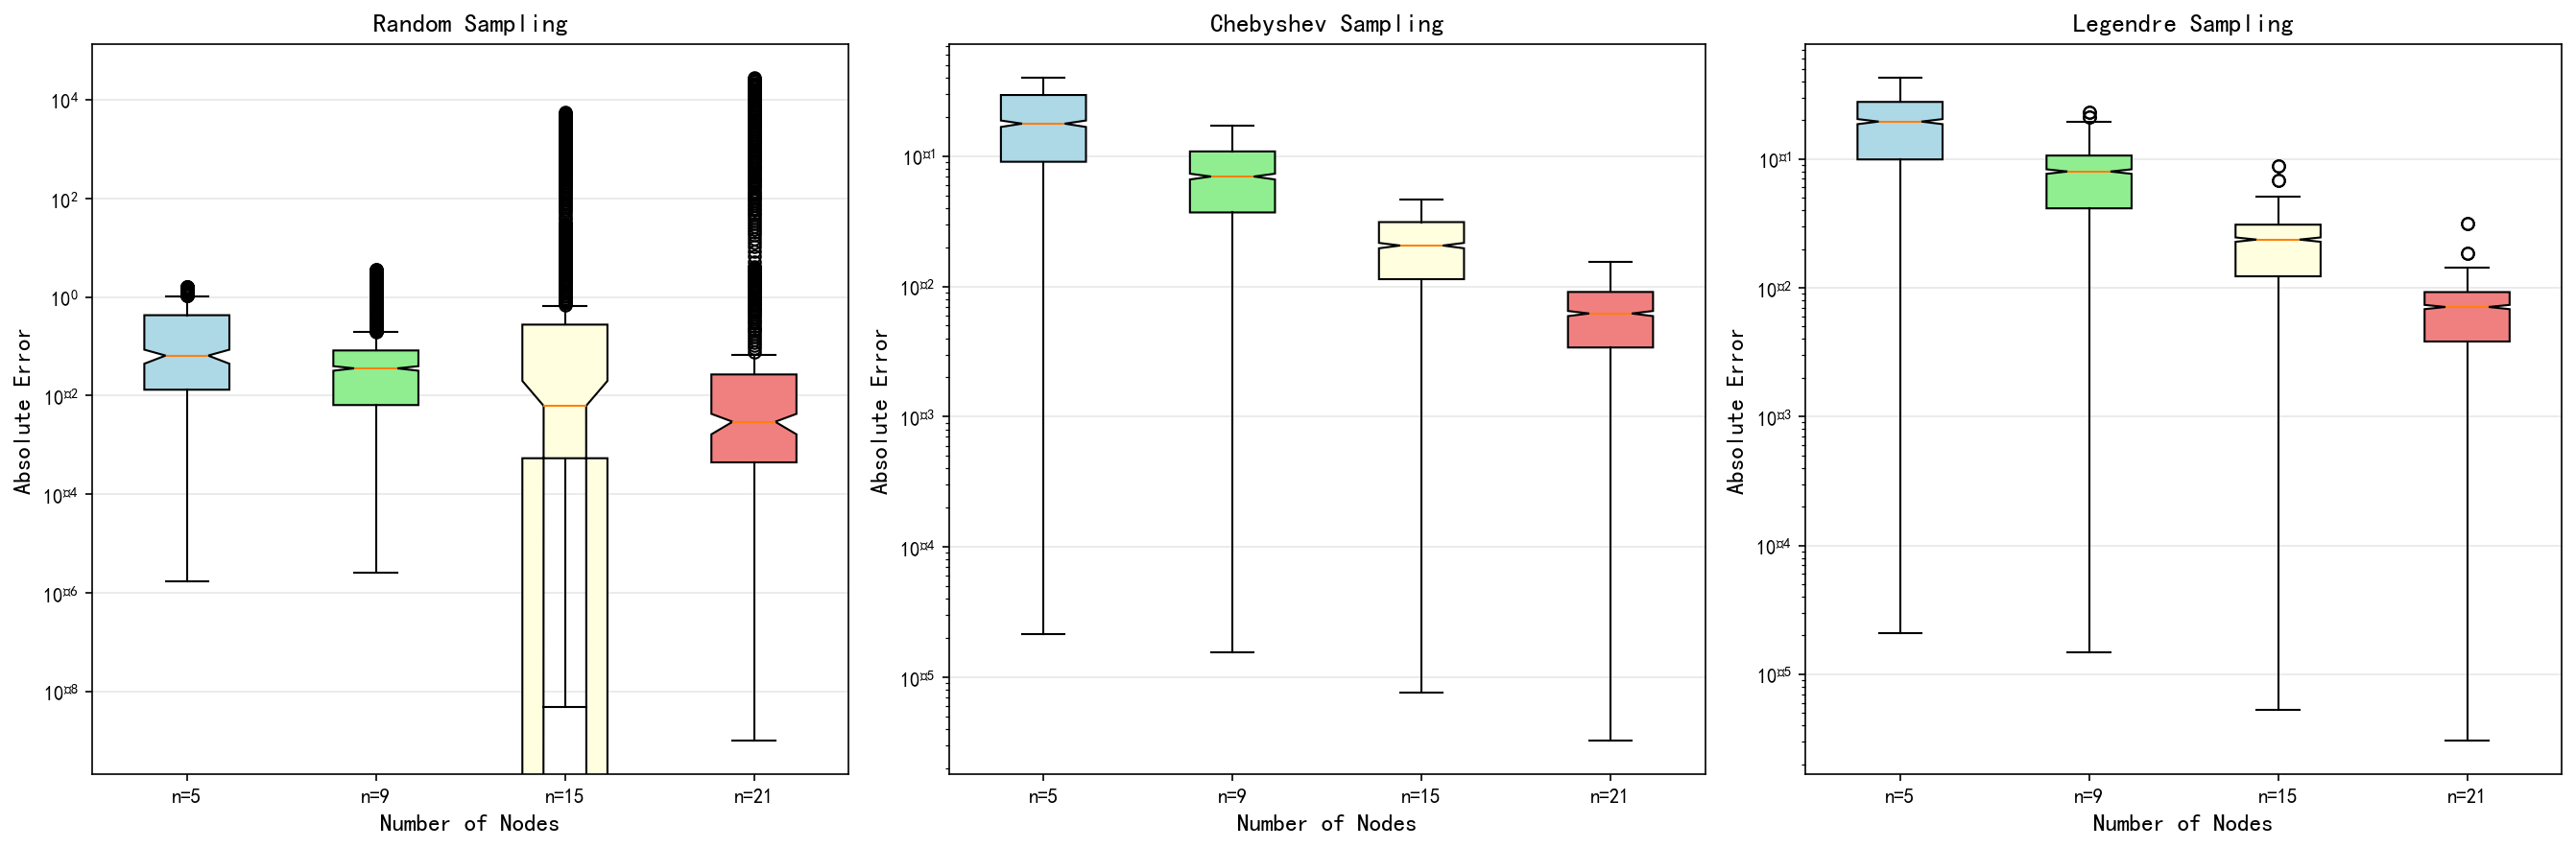
\includegraphics[width=0.95\textwidth]{results/task1/additional/error_boxplot.png}
\caption{三种采样策略的误差箱线图对比}
\label{fig:task1_error_boxplot}
\end{figure}

图\ref{fig:task1_error_boxplot}通过箱线图展示误差的统计特性:
\begin{itemize}
    \item \textbf{中位数}:切比雪夫和勒让德节点的误差中位数随$n$单调递减
    \item \textbf{四分位距}:随机采样的四分位距随$n$急剧增大,显示误差波动极大
    \item \textbf{异常值}:随机采样在$n=15, 21$时出现大量异常值(上界外的点)
\end{itemize}

\subsection{收敛性分析}

\begin{figure}[H]
\centering
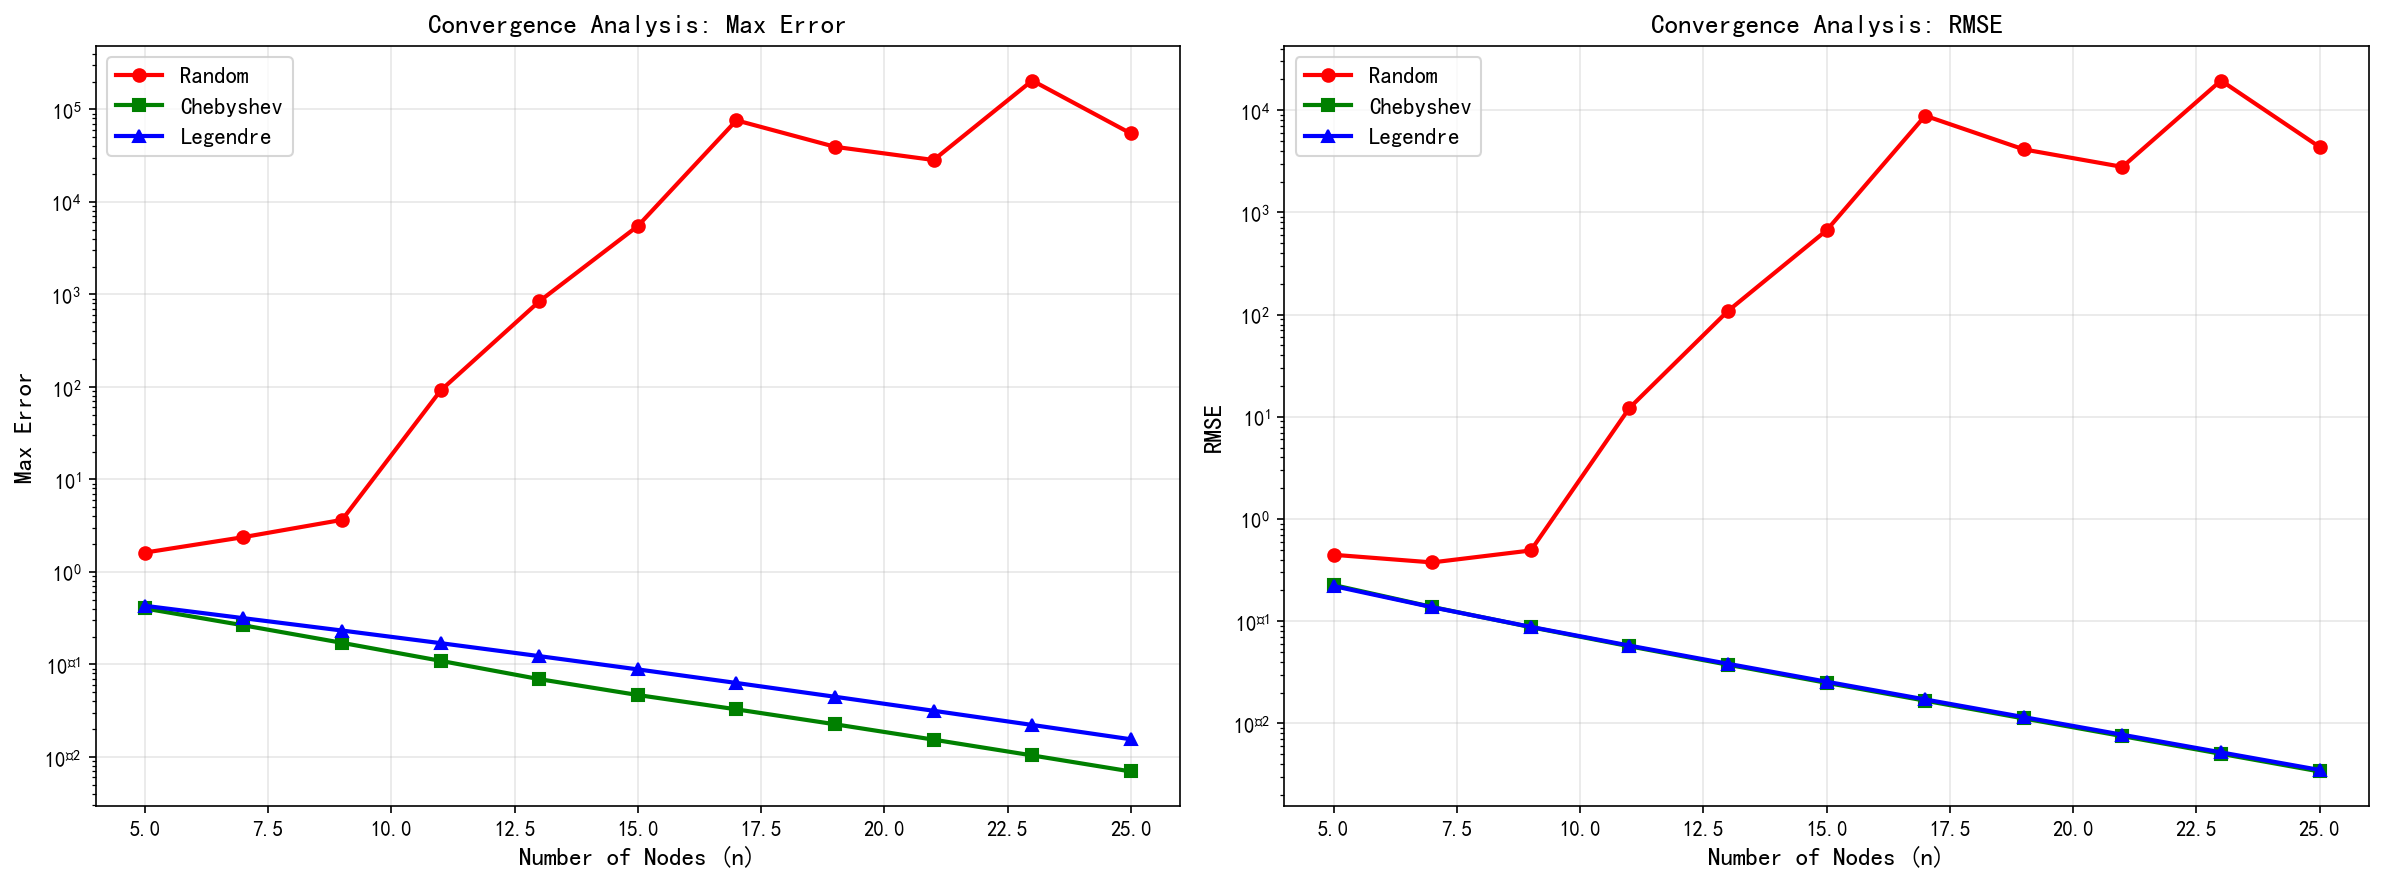
\includegraphics[width=0.95\textwidth]{results/task1/additional/convergence_analysis.png}
\caption{插值误差随节点数的收敛曲线}
\label{fig:task1_convergence}
\end{figure}

图\ref{fig:task1_convergence}量化展示了三种方法的收敛性:
\begin{itemize}
    \item \textbf{切比雪夫节点}:呈现理想的指数收敛特性(直线下降)
    \item \textbf{勒让德节点}:收敛速度略慢于切比雪夫,但同样稳定
    \item \textbf{随机采样}:$n<10$时有所收敛,$n>10$后发散(曲线上扬)
\end{itemize}

\newpage
\section{任务二:最小二乘法曲线拟合}

\subsection{实验设置}

\subsubsection{目标函数}

\begin{equation}
g(x) = c\sin(dx) + e\cos(fx) = 2.0\sin(1.5x) + 1.5\cos(2.5x)
\end{equation}

其中参数设置为:
\begin{equation}
c = 2.0, \quad d = 1.5, \quad e = 1.5, \quad f = 2.5
\end{equation}

\subsubsection{实验参数}

\begin{table}[h]
\centering
\caption{任务二实验参数}
\begin{tabular}{ll}
\toprule
\textbf{参数} & \textbf{值} \\
\midrule
区间 & $[0, 2\pi]$ \\
采样点数 & 81 \\
测试点数 & 100 \\
基函数 & $\{\sin(1.5x), \cos(2.5x)\}$ \\
\bottomrule
\end{tabular}
\end{table}

\subsection{子任务1:扰动影响分析}

\subsubsection{扰动模型}

对采样点$y$值添加扰动:

\begin{equation}
\tilde{y}_i = y_i + \delta_i, \quad \delta_i \sim U(-\alpha y_i, \alpha y_i)
\end{equation}

其中$\alpha \in \{0\%, 10\%, 20\%, 30\%\}$为扰动水平。

\subsubsection{实验结果}

\begin{table}[H]
\centering
\caption{扰动对拟合精度的影响}
\begin{tabular}{lrrr}
\toprule
\textbf{扰动水平} & \textbf{RMSE} & \textbf{MAE} & \textbf{系数误差} \\
\midrule
No Perturbation & 4.947e-16 & 3.847e-16 & 8.882e-16 \\
Perturbation 10\% & 2.144e-02 & 1.800e-02 & 4.215e-02 \\
Perturbation 20\% & 8.397e-03 & 6.833e-03 & 1.678e-02 \\
Perturbation 30\% & 4.142e-02 & 3.458e-02 & 8.185e-02 \\
\bottomrule
\end{tabular}
\end{table}

图\ref{fig:task2_subtask1}展示了不同扰动水平下的拟合结果:

\begin{figure}[H]
\centering
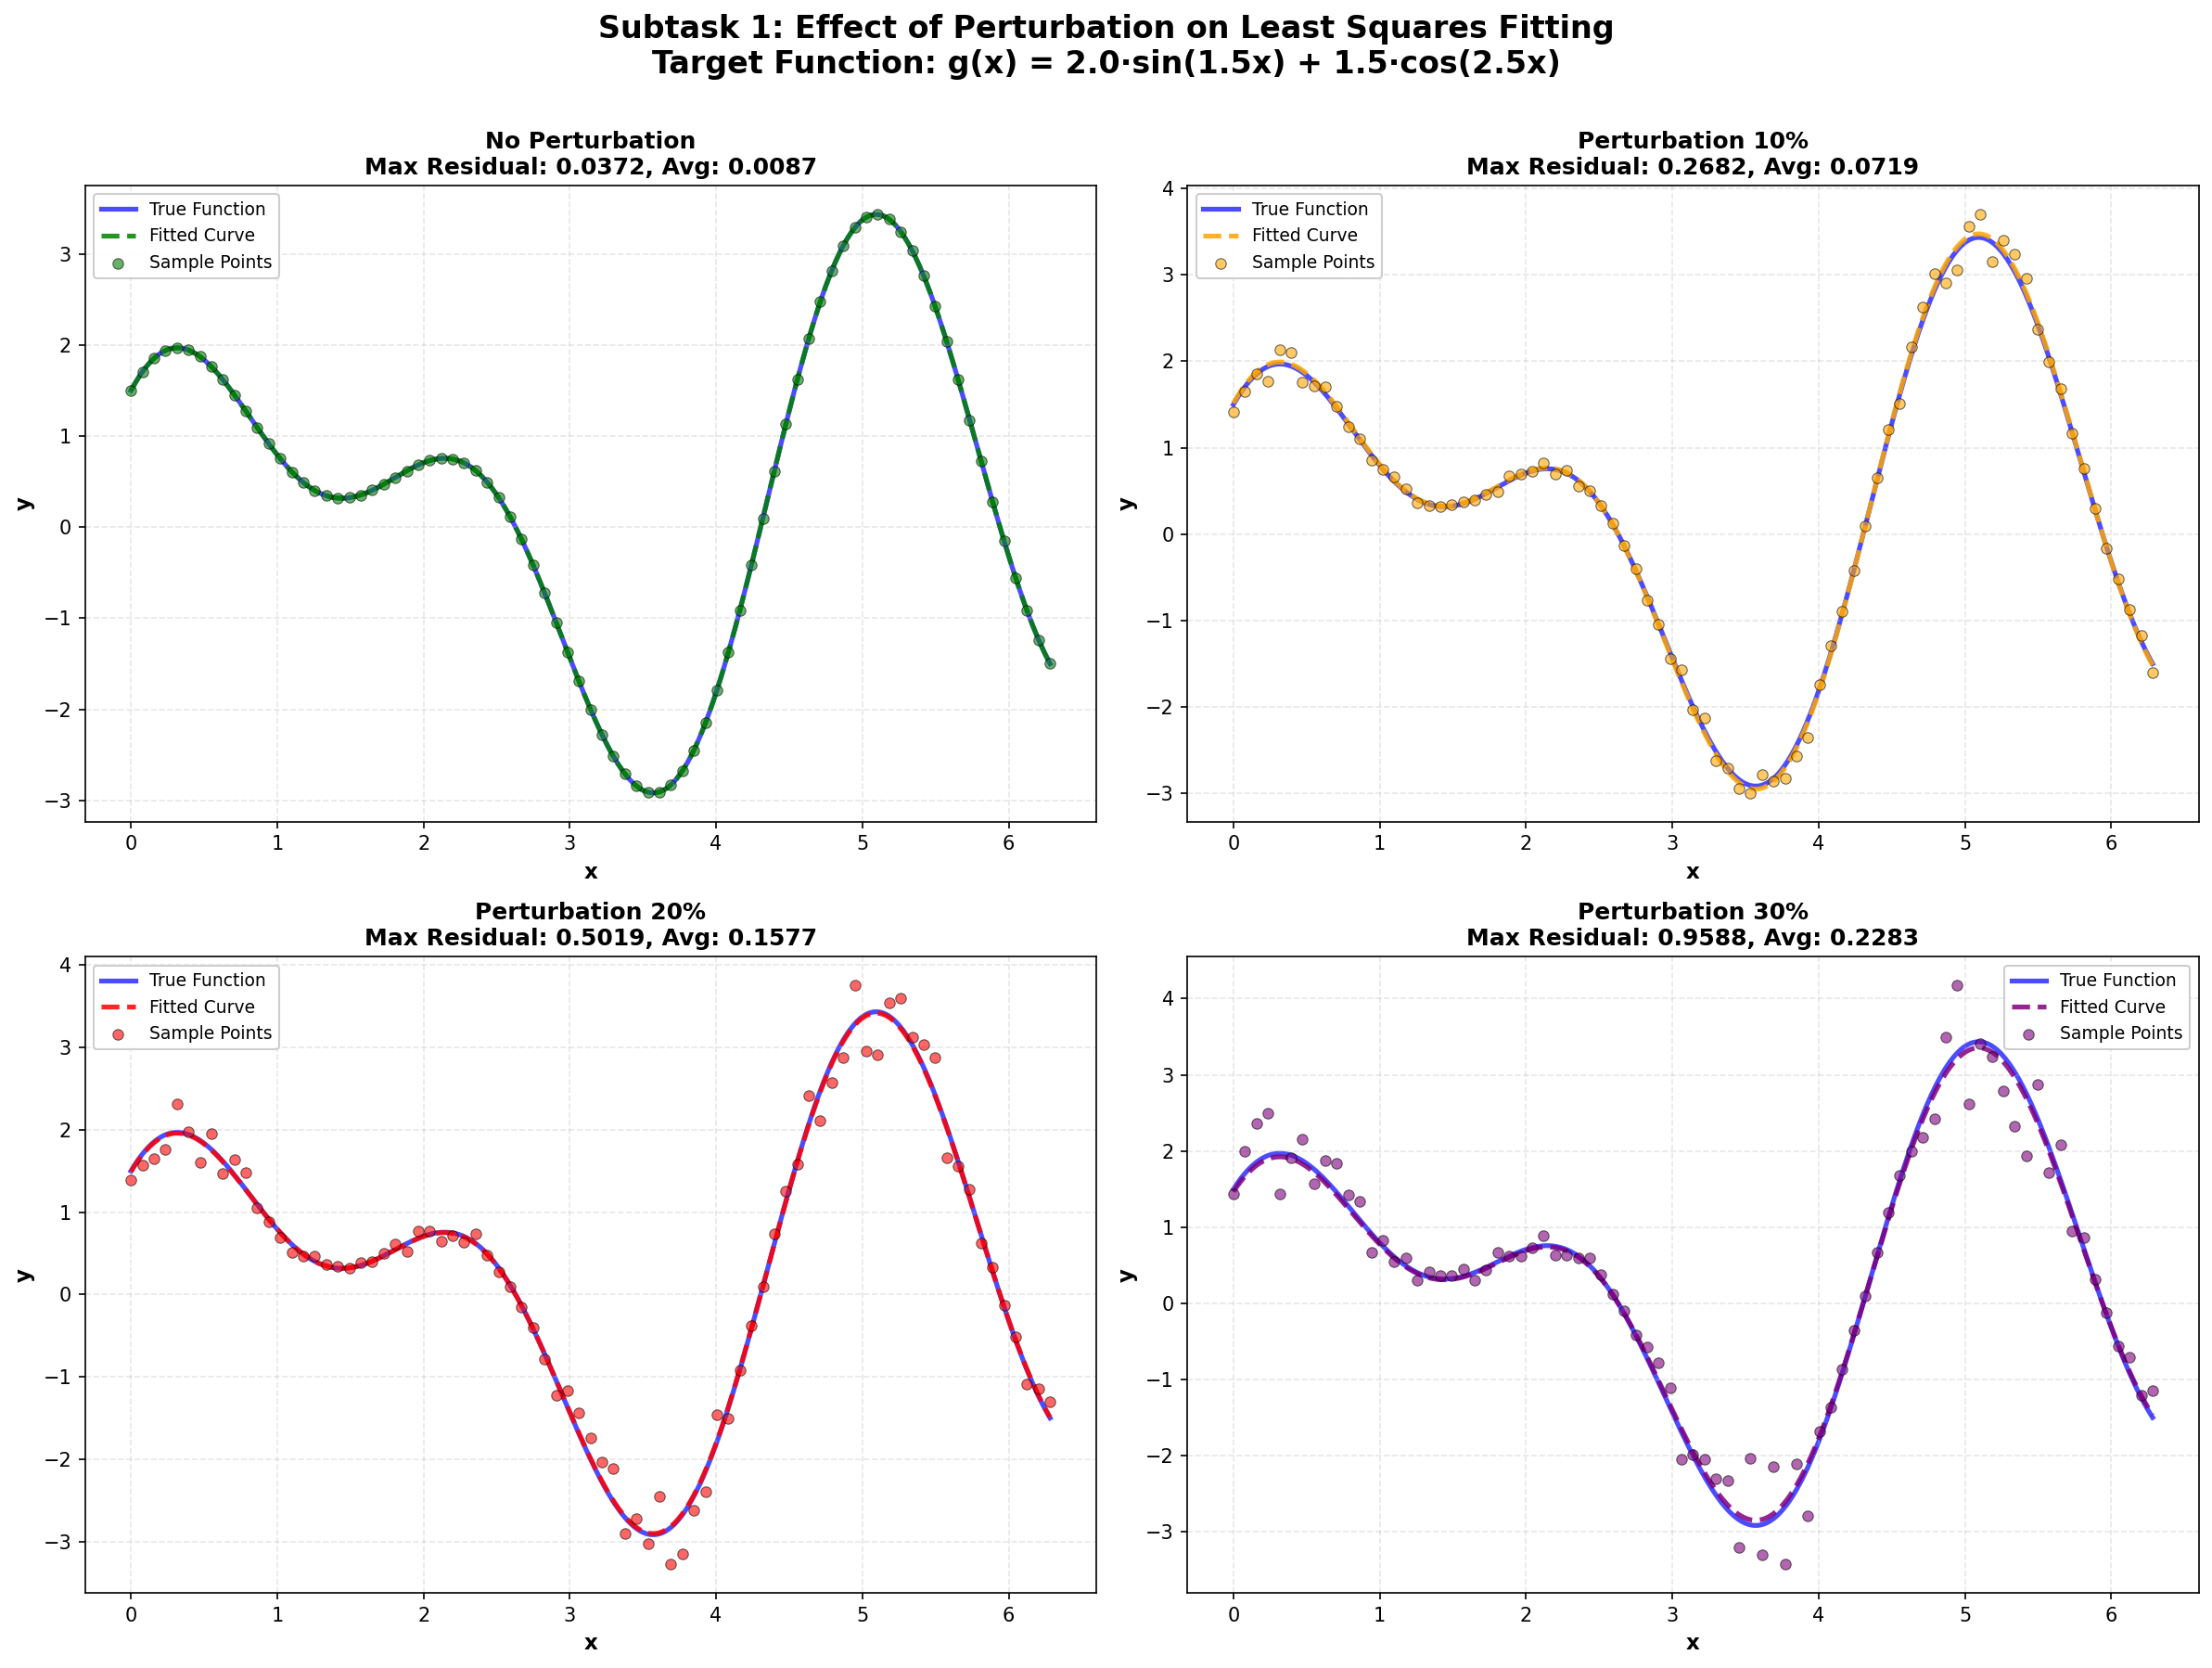
\includegraphics[width=0.95\textwidth]{results/task2/subtask1/comprehensive_comparison.png}
\caption{子任务1:扰动对最小二乘拟合的影响}
\label{fig:task2_subtask1}
\end{figure}

\textbf{观察}:
\begin{itemize}
    \item 无扰动时RMSE达到机器精度($\sim 10^{-16}$),说明拟合完美
    \item 扰动导致误差线性增长,但仍在可接受范围
    \item 系数误差与扰动水平基本成正比
    \item 即使30\%扰动下,拟合曲线仍能较好地跟踪真实函数
\end{itemize}

\subsubsection{残差分析}

为了进一步分析拟合质量,我们绘制了残差图:

\begin{figure}[H]
\centering
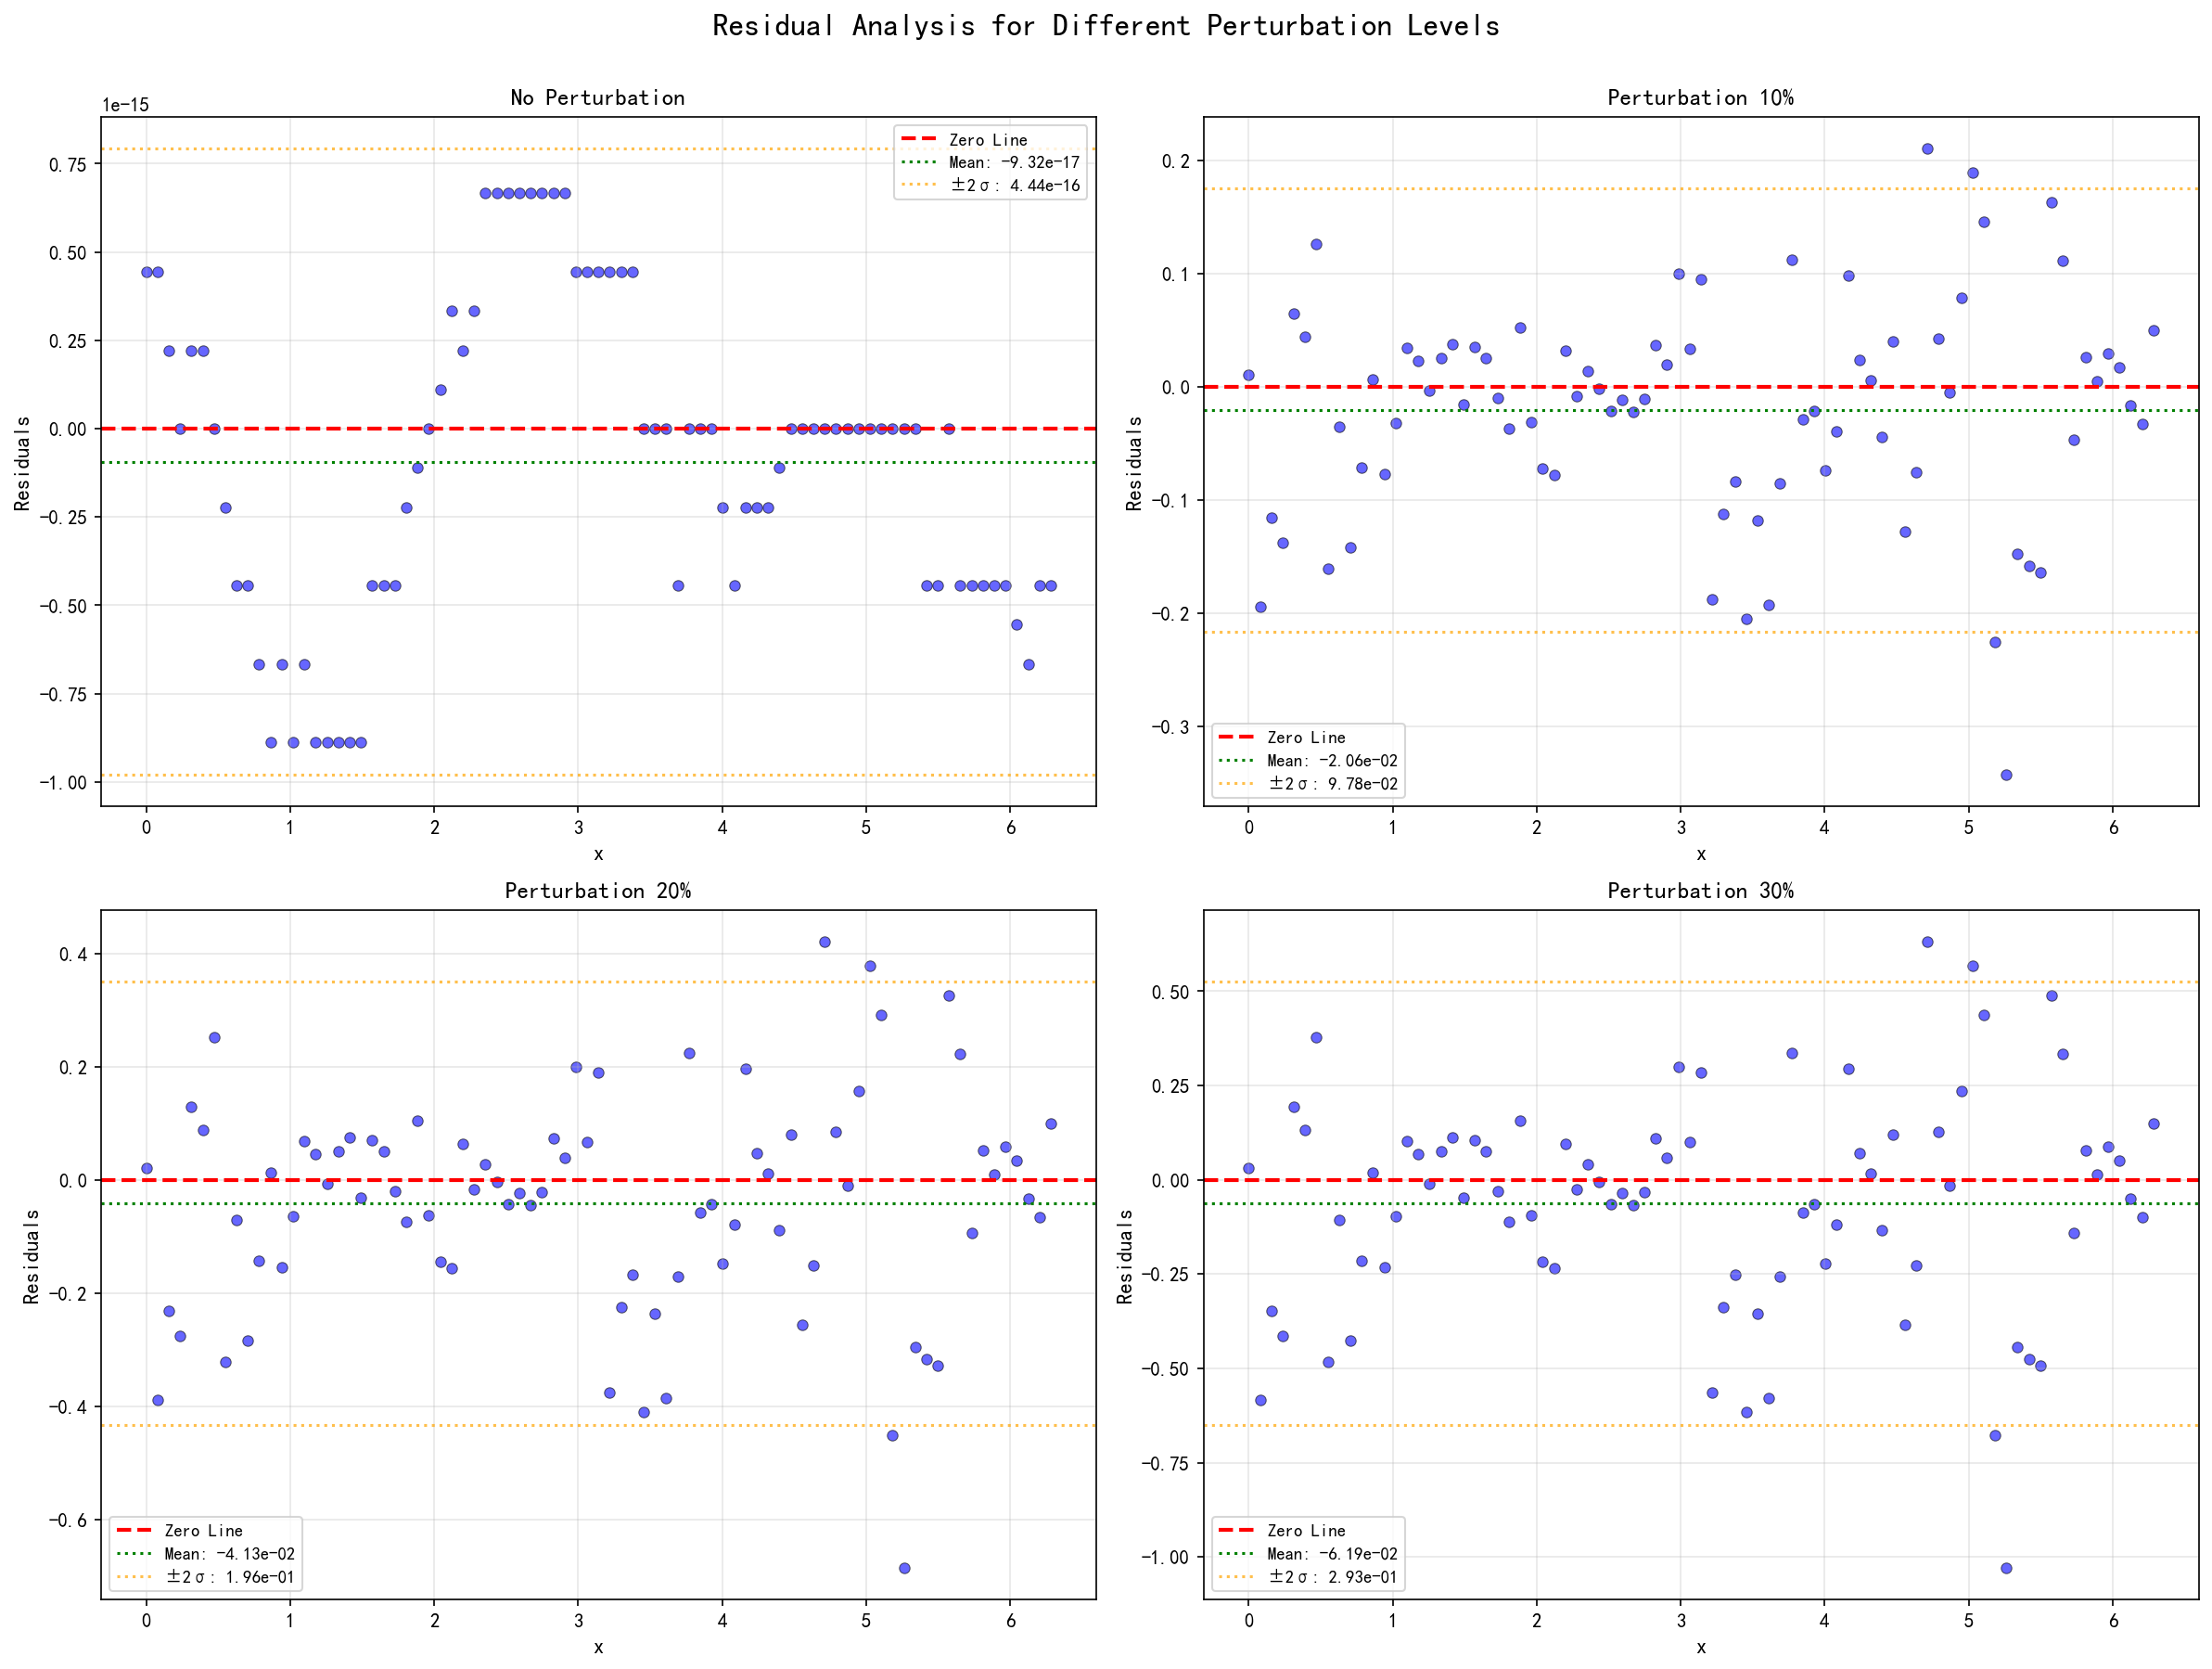
\includegraphics[width=0.95\textwidth]{results/task2/additional/residual_analysis.png}
\caption{不同扰动水平下的残差分析}
\label{fig:task2_residual}
\end{figure}

图\ref{fig:task2_residual}展示了残差的分布特征:
\begin{itemize}
    \item \textbf{无扰动}:残差接近零线,分布在机器精度范围内($\sim 10^{-15}$)
    \item \textbf{有扰动}:残差均匀分布在零线两侧,无明显模式(表明模型选择正确)
    \item \textbf{均值}:所有情况下残差均值接近零(绿色虚线)
    \item \textbf{标准差}:随扰动水平增大而增大(橙色虚线为$\pm 2\sigma$)
\end{itemize}

\subsubsection{系数误差分析}

\begin{figure}[H]
\centering
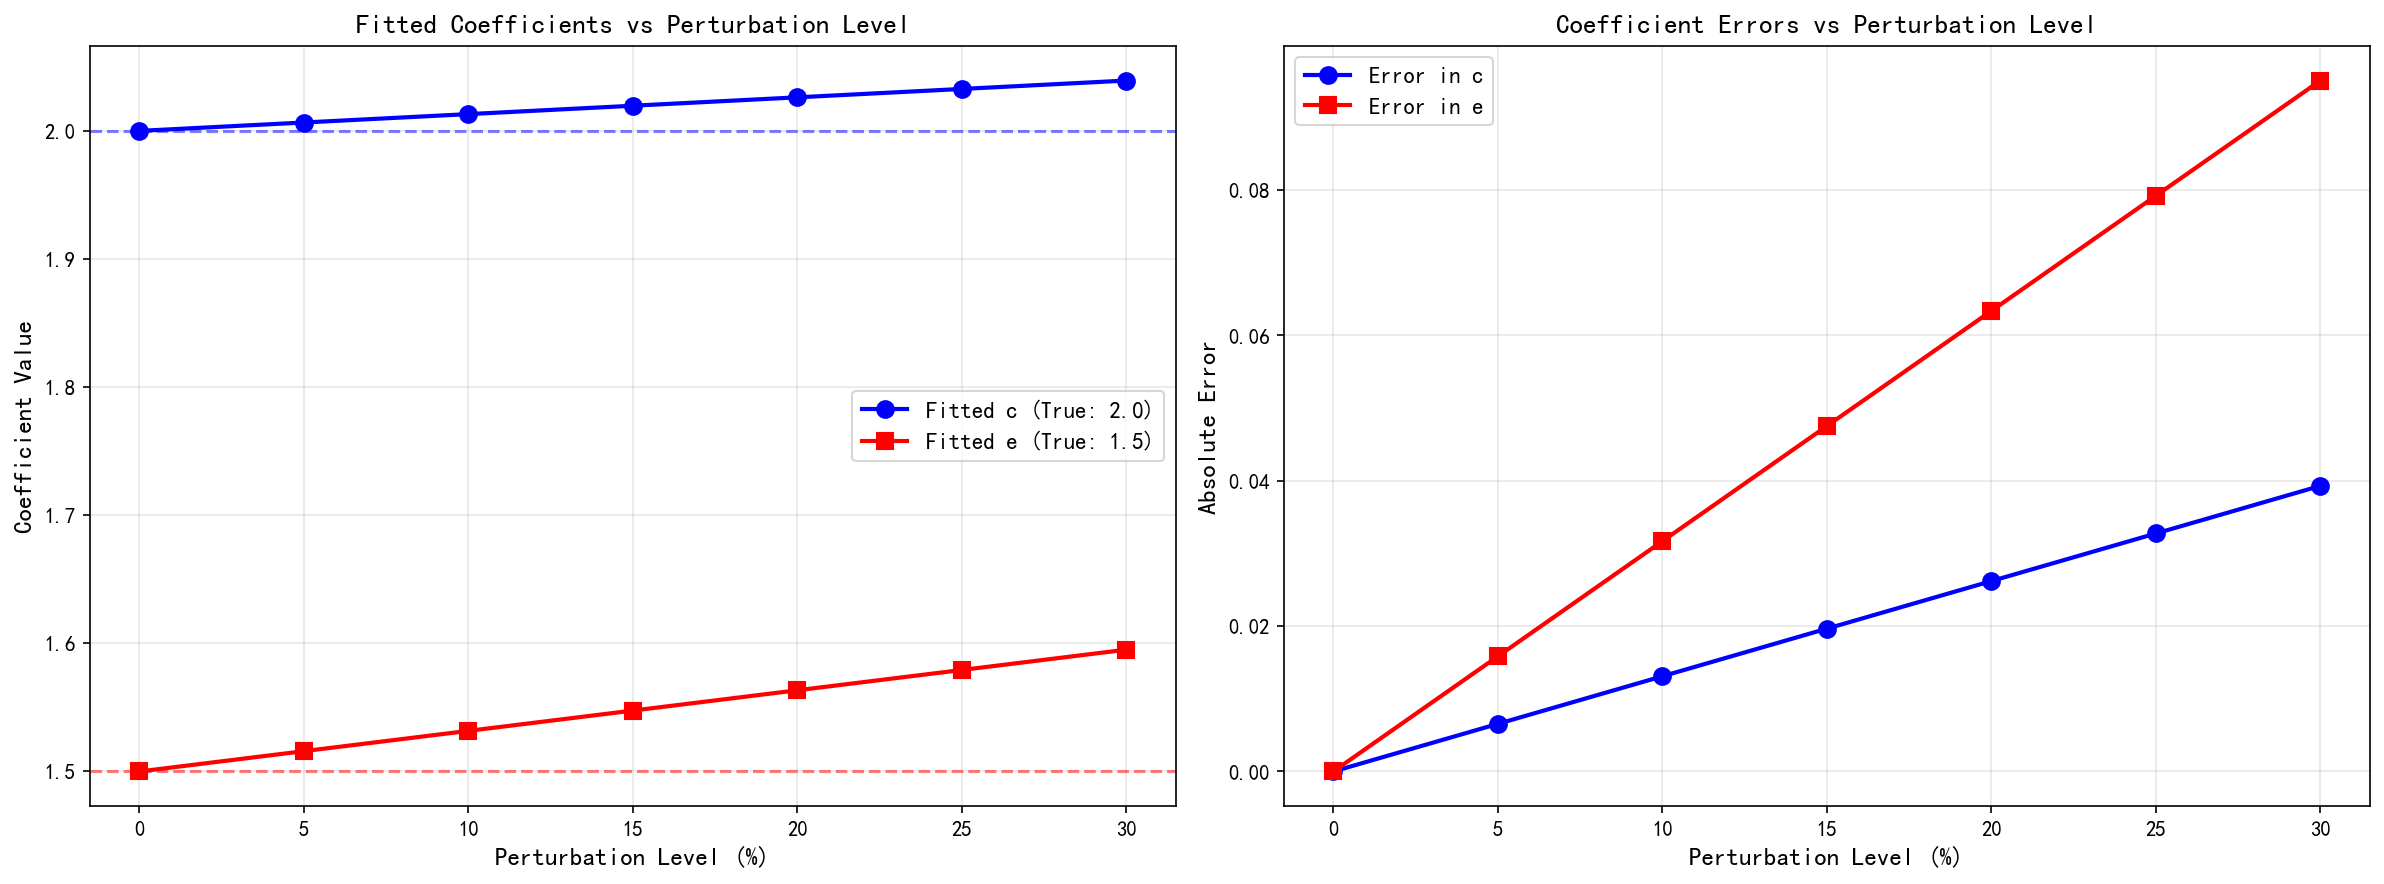
\includegraphics[width=0.95\textwidth]{results/task2/additional/coefficient_analysis.png}
\caption{拟合系数随扰动水平的变化}
\label{fig:task2_coeff}
\end{figure}

图\ref{fig:task2_coeff}定量展示了扰动对拟合系数的影响:
\begin{itemize}
    \item \textbf{左图}:拟合系数值随扰动水平的变化
    \begin{itemize}
        \item 无扰动时,拟合系数完美重合于真实值(水平虚线)
        \item 扰动导致系数轻微偏离,但整体趋势稳定
    \end{itemize}
    \item \textbf{右图}:系数绝对误差
    \begin{itemize}
        \item 误差与扰动水平呈近似线性关系
        \item 30\%扰动下,系数误差约为0.08(相对真实值约4\%)
    \end{itemize}
\end{itemize}

\subsection{子任务2:分段多项式拟合}

\subsubsection{实验设计}

将区间$[0, 2\pi]$等分为2、4、8段,在每段使用1、2、3、4次多项式拟合,共12种配置。

\subsubsection{误差矩阵}

\begin{table}[H]
\centering
\caption{分段多项式拟合误差矩阵(RMSE)}
\begin{tabular}{lrrrr}
\toprule
\textbf{分段数} & \textbf{Degree 1} & \textbf{Degree 2} & \textbf{Degree 3} & \textbf{Degree 4} \\
\midrule
2 Segments & 1.3466 & 0.8408 & 0.4584 & 0.1888 \\
4 Segments & 0.5639 & 0.1893 & 0.0484 & 0.0100 \\
\rowcolor{tablerowcolor}
8 Segments & 0.1628 & 0.0319 & 0.0037 & \textbf{0.0006} \\
\bottomrule
\end{tabular}
\end{table}

\textbf{最佳配置}:8分段 + 4次多项式,RMSE = 6.492e-04

图\ref{fig:task2_subtask2_heatmap}展示了误差矩阵的热力图:

\begin{figure}[H]
\centering
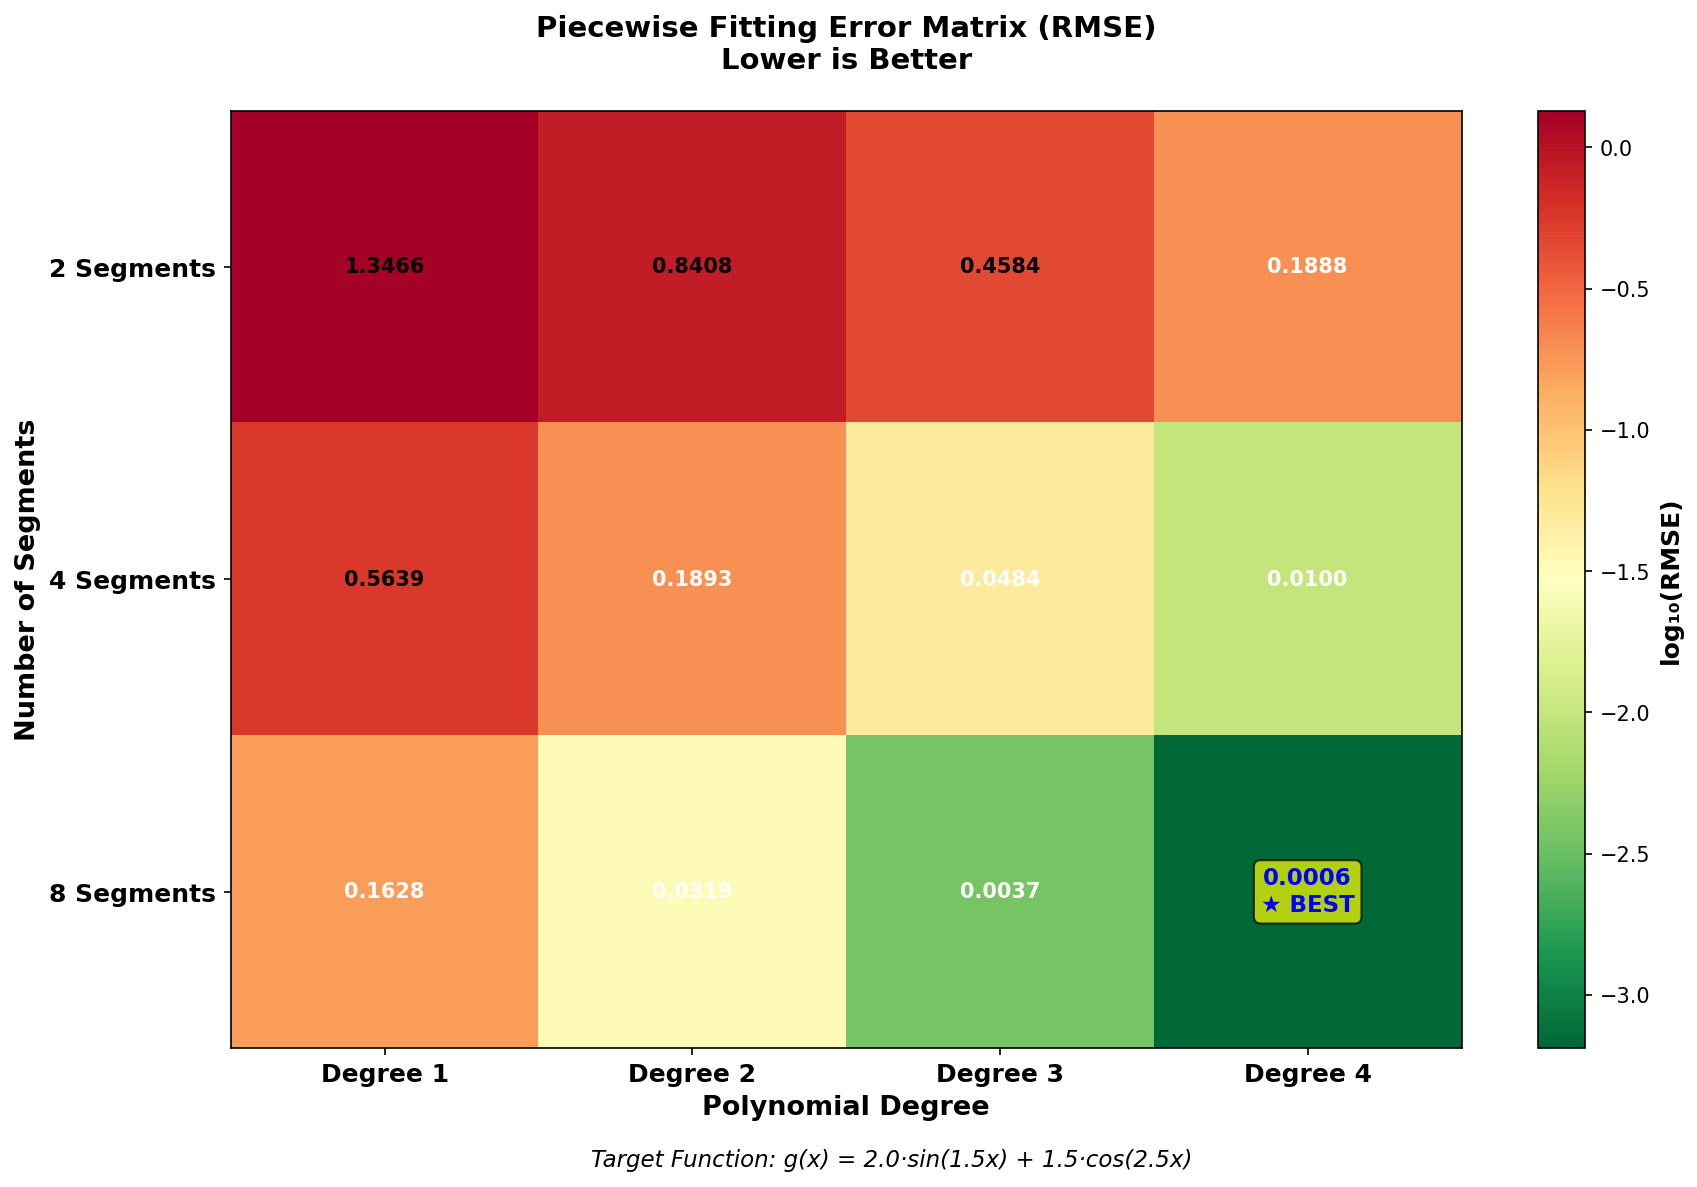
\includegraphics[width=0.7\textwidth]{results/task2/subtask2/error_heatmap.png}
\caption{子任务2:分段多项式拟合误差热力图}
\label{fig:task2_subtask2_heatmap}
\end{figure}

图\ref{fig:task2_subtask2_segments}展示了不同分段数下各多项式次数的拟合效果对比:

\begin{figure}[H]
\centering
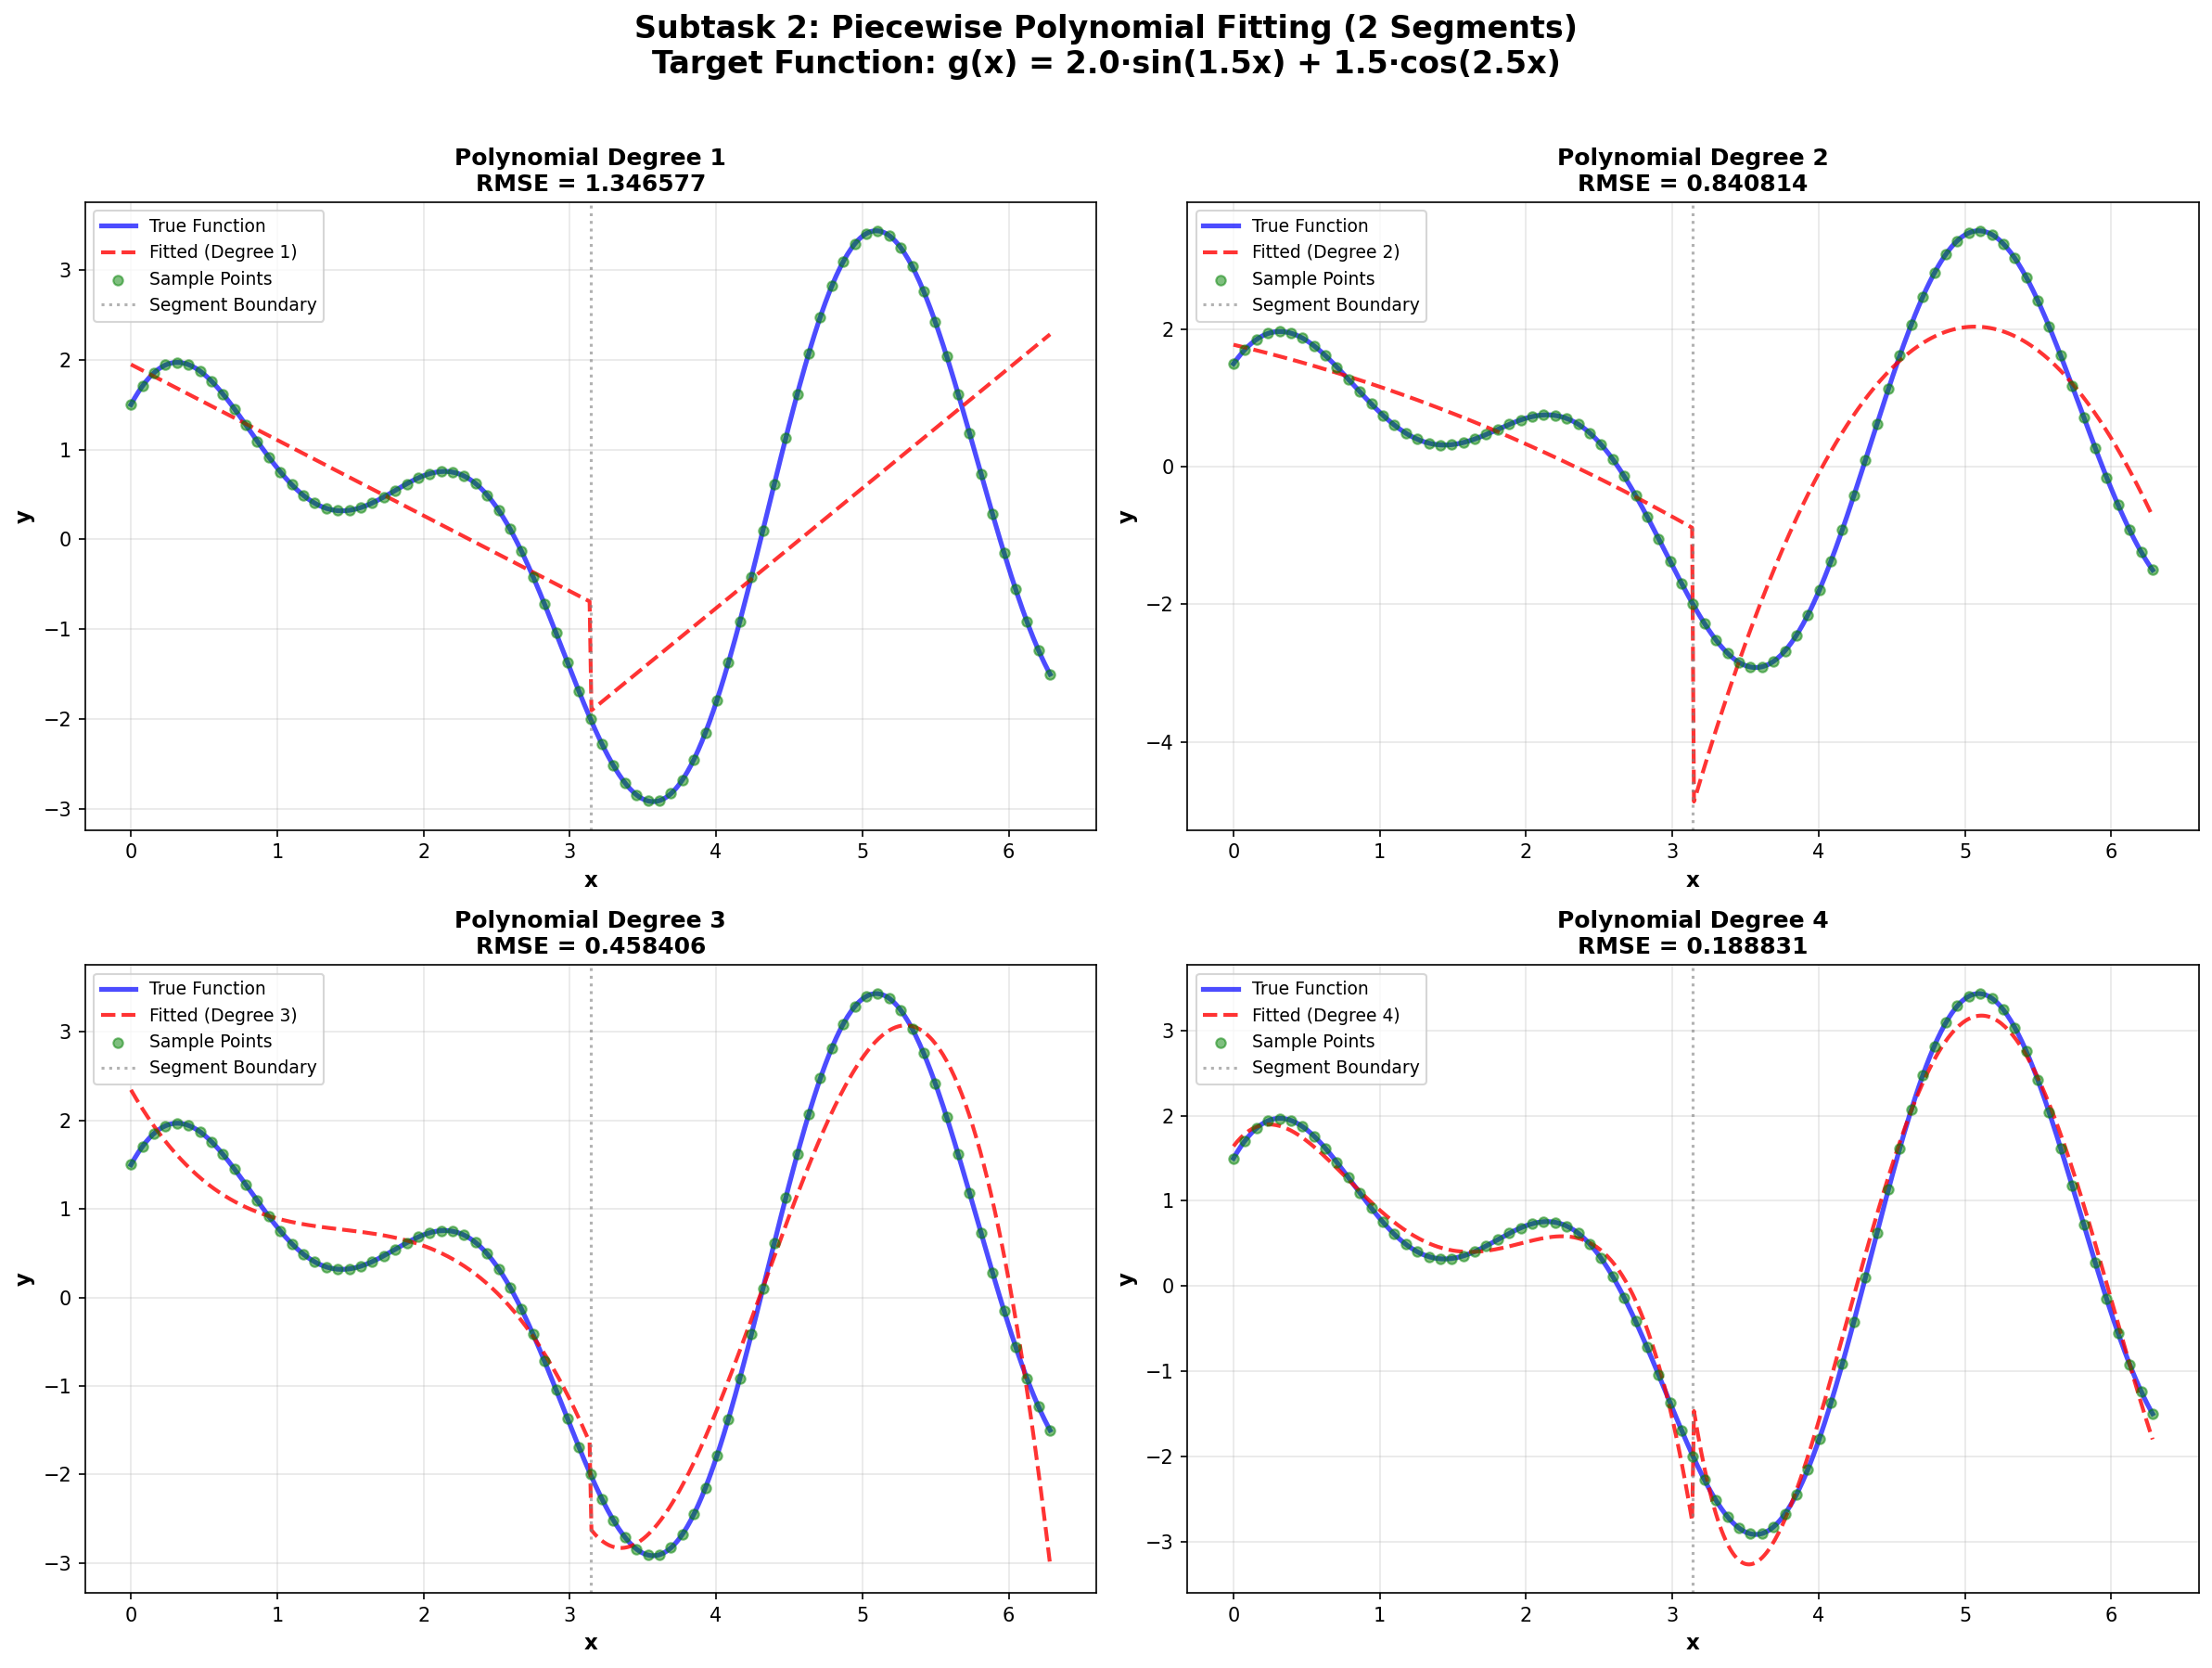
\includegraphics[width=0.48\textwidth]{results/task2/subtask2/comparison_2_segments.png}
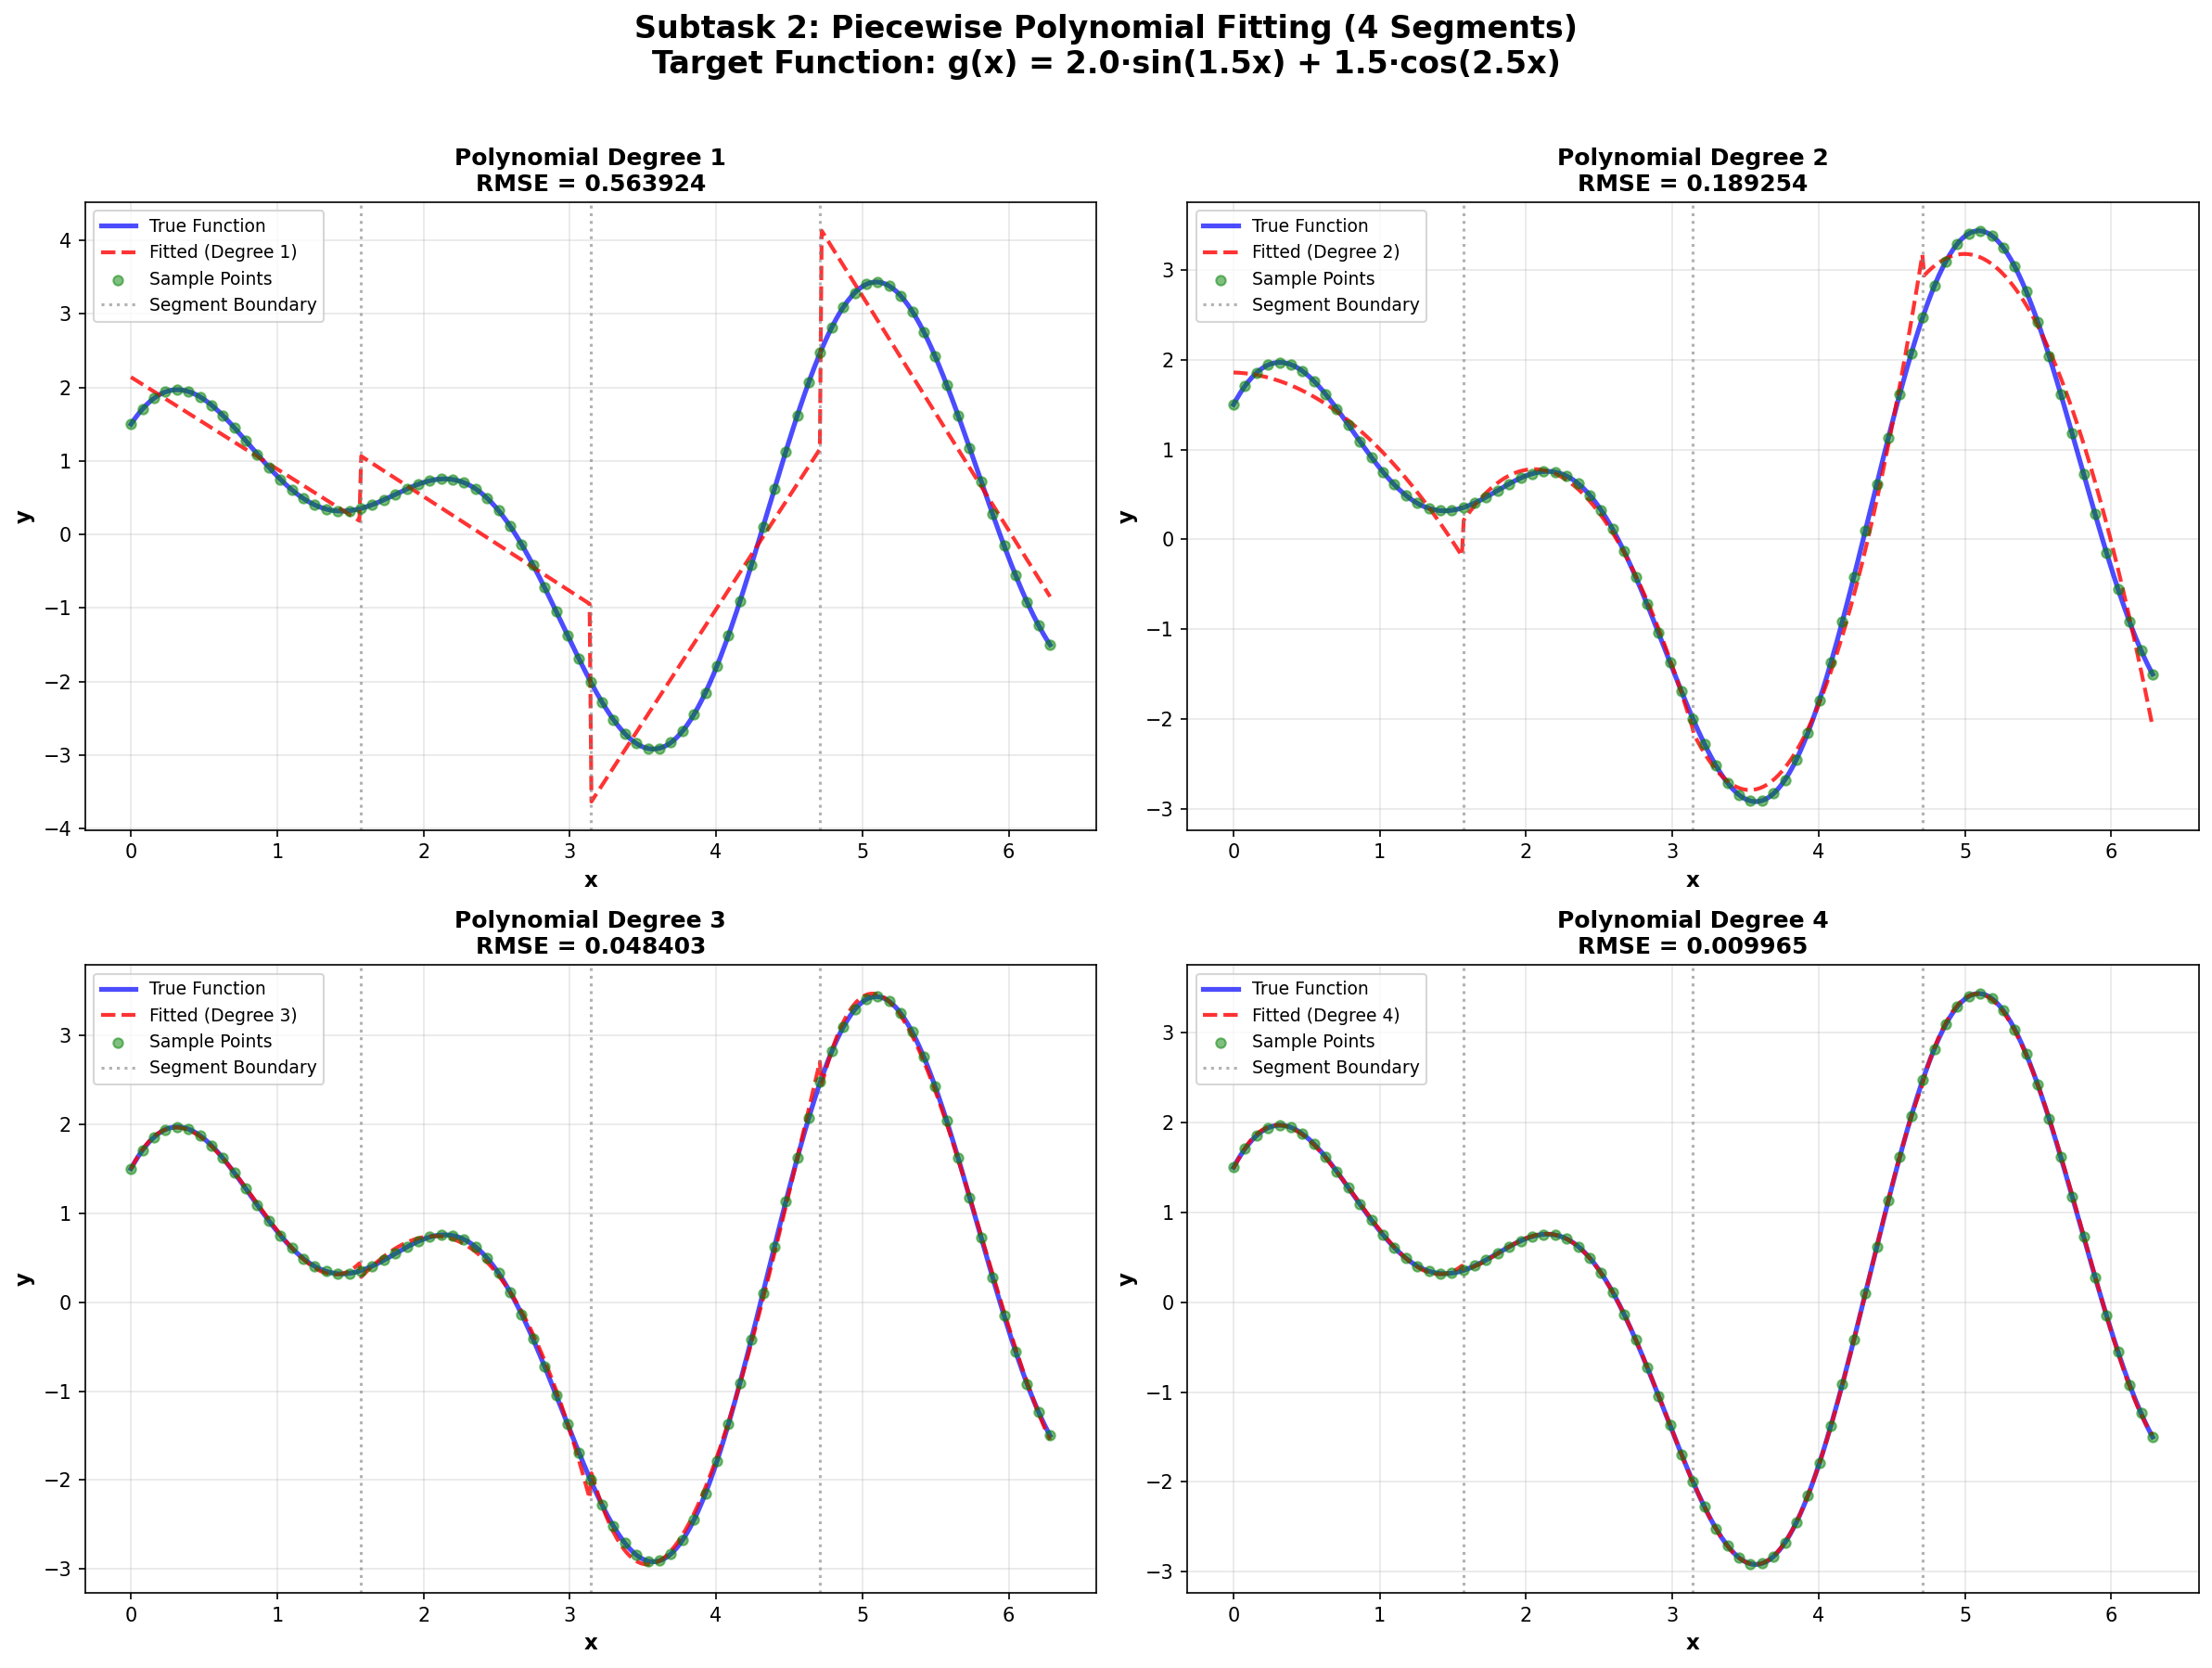
\includegraphics[width=0.48\textwidth]{results/task2/subtask2/comparison_4_segments.png}
\caption{2分段(左)和4分段(右)的多项式拟合对比}
\label{fig:task2_subtask2_segments}
\end{figure}

\begin{figure}[H]
\centering
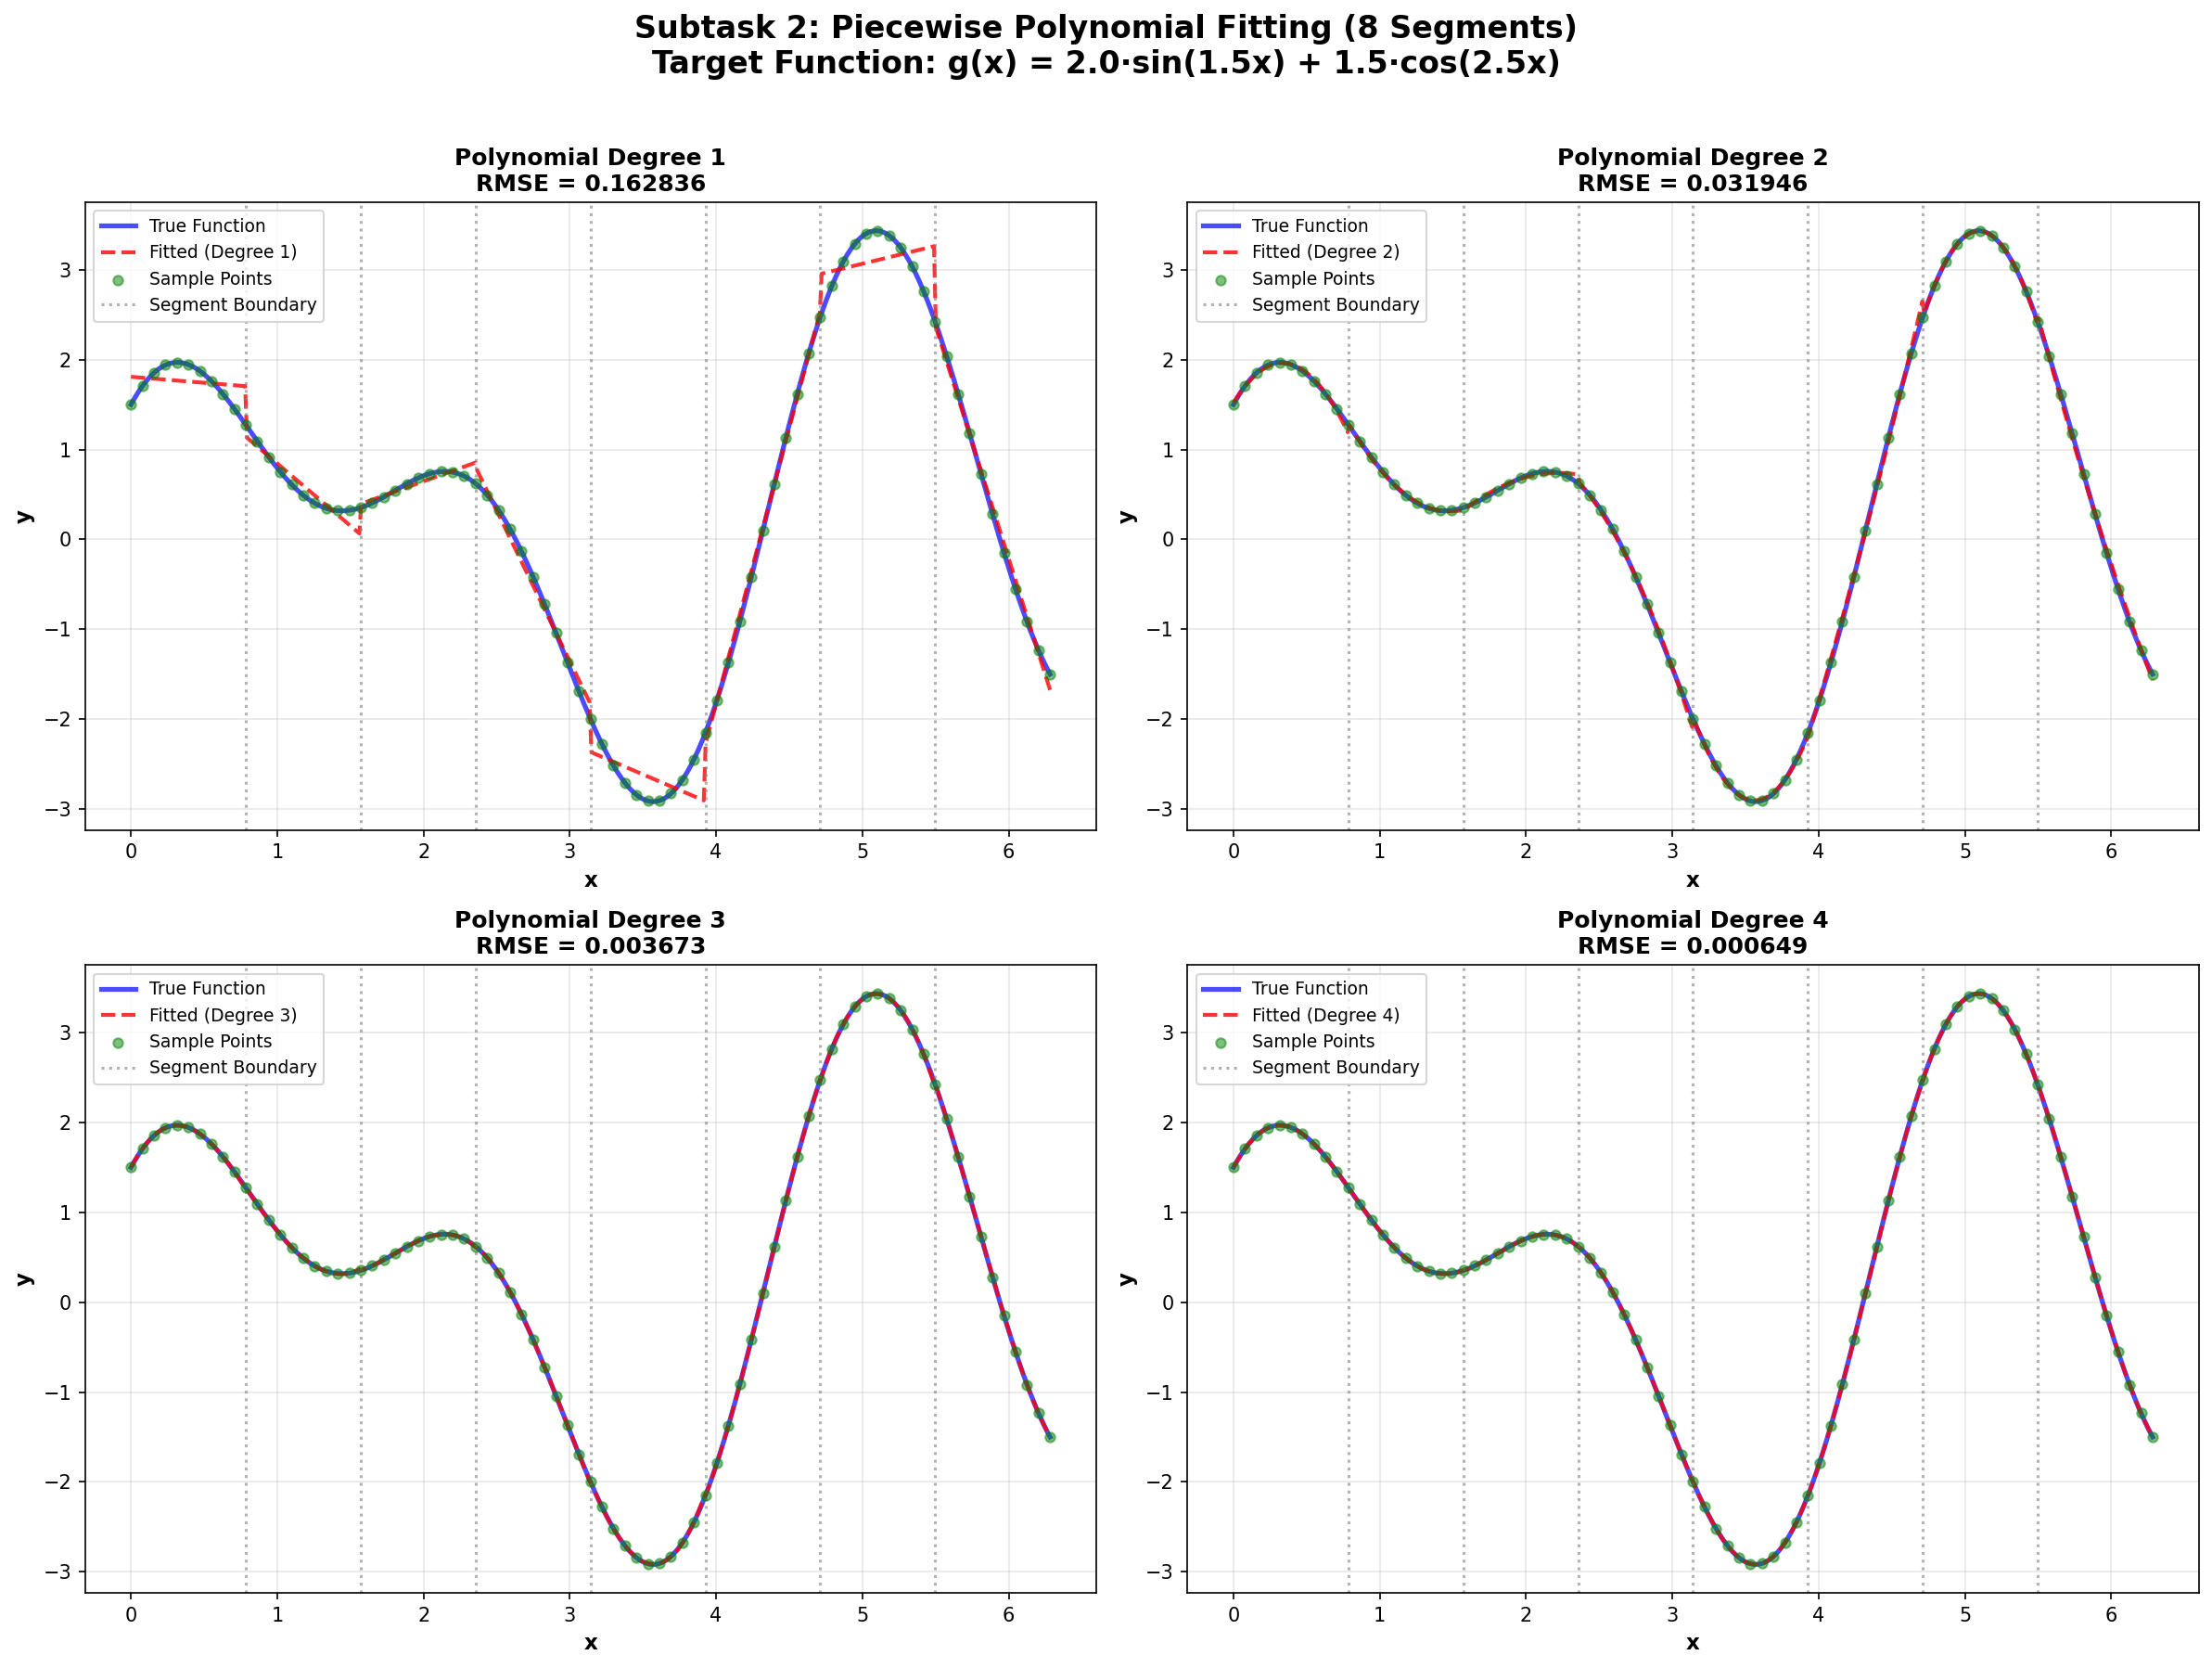
\includegraphics[width=0.9\textwidth]{results/task2/subtask2/comparison_8_segments.png}
\caption{8分段的多项式拟合对比(最佳配置)}
\label{fig:task2_subtask2_8seg}
\end{figure}

从图\ref{fig:task2_subtask2_segments}和图\ref{fig:task2_subtask2_8seg}可以清晰看到:
\begin{itemize}
    \item \textbf{2分段}:只能粗略逼近目标函数,即使4次多项式也存在明显误差
    \item \textbf{4分段}:逼近质量显著提升,3-4次多项式效果良好
    \item \textbf{8分段}:各次多项式都能较好拟合,4次多项式达到最优精度
    \item 分段边界处连续性保持良好
\end{itemize}

\subsubsection{规律总结}

\begin{enumerate}
    \item \textbf{分段数影响}:分段数从2增加到8,误差显著降低(局部逼近更精确)
    \item \textbf{多项式次数影响}:
    \begin{itemize}
        \item 2分段时:受限于点数,高次多项式优势不明显
        \item 8分段时:随次数增加误差单调递减
    \end{itemize}
    \item \textbf{过拟合风险}:8分段+4次时每段约10个点,接近过拟合边界
\end{enumerate}

\subsection{子任务3:RANSAC鲁棒拟合}

\subsubsection{噪声模型}

测试三种噪声场景:
\begin{enumerate}
    \item \textbf{高斯噪声}:$\epsilon \sim N(0, (0.2 \cdot \text{range})^2)$
    \item \textbf{离群点}:25\%的点被大幅扰动
    \item \textbf{混合噪声}:高斯噪声 + 20\%离群点
\end{enumerate}

\subsubsection{RANSAC参数}

\begin{table}[h]
\centering
\caption{RANSAC算法参数设置}
\begin{tabular}{lrrr}
\toprule
\textbf{参数} & \textbf{高斯噪声} & \textbf{离群点} & \textbf{混合噪声} \\
\midrule
最大迭代次数 & 1500 & 1500 & 1500 \\
内点阈值$\tau$ & 0.3 & 0.5 & 0.4 \\
最小样本数 & 5 & 5 & 5 \\
\bottomrule
\end{tabular}
\end{table}

\subsubsection{实验结果}

\begin{table}[H]
\centering
\caption{RANSAC vs 标准最小二乘(RMSE对比)}
\begin{tabular}{lrrr}
\toprule
\textbf{噪声类型} & \textbf{标准LS} & \textbf{RANSAC} & \textbf{改善率} \\
\midrule
高斯噪声 & 0.3165 & 0.7930 & -150.59\% \\
\rowcolor{tablerowcolor}
离群点 & 1.2978 & 0.0112 & \textbf{+99.14\%} \\
\rowcolor{tablerowcolor}
混合噪声 & 1.6654 & 0.2530 & \textbf{+84.81\%} \\
\bottomrule
\end{tabular}
\end{table}

\subsubsection{可视化结果}

为了更清晰地展示RANSAC在不同噪声场景下的表现,我们分别展示了三种噪声类型的详细对比图。

\begin{figure}[H]
\centering
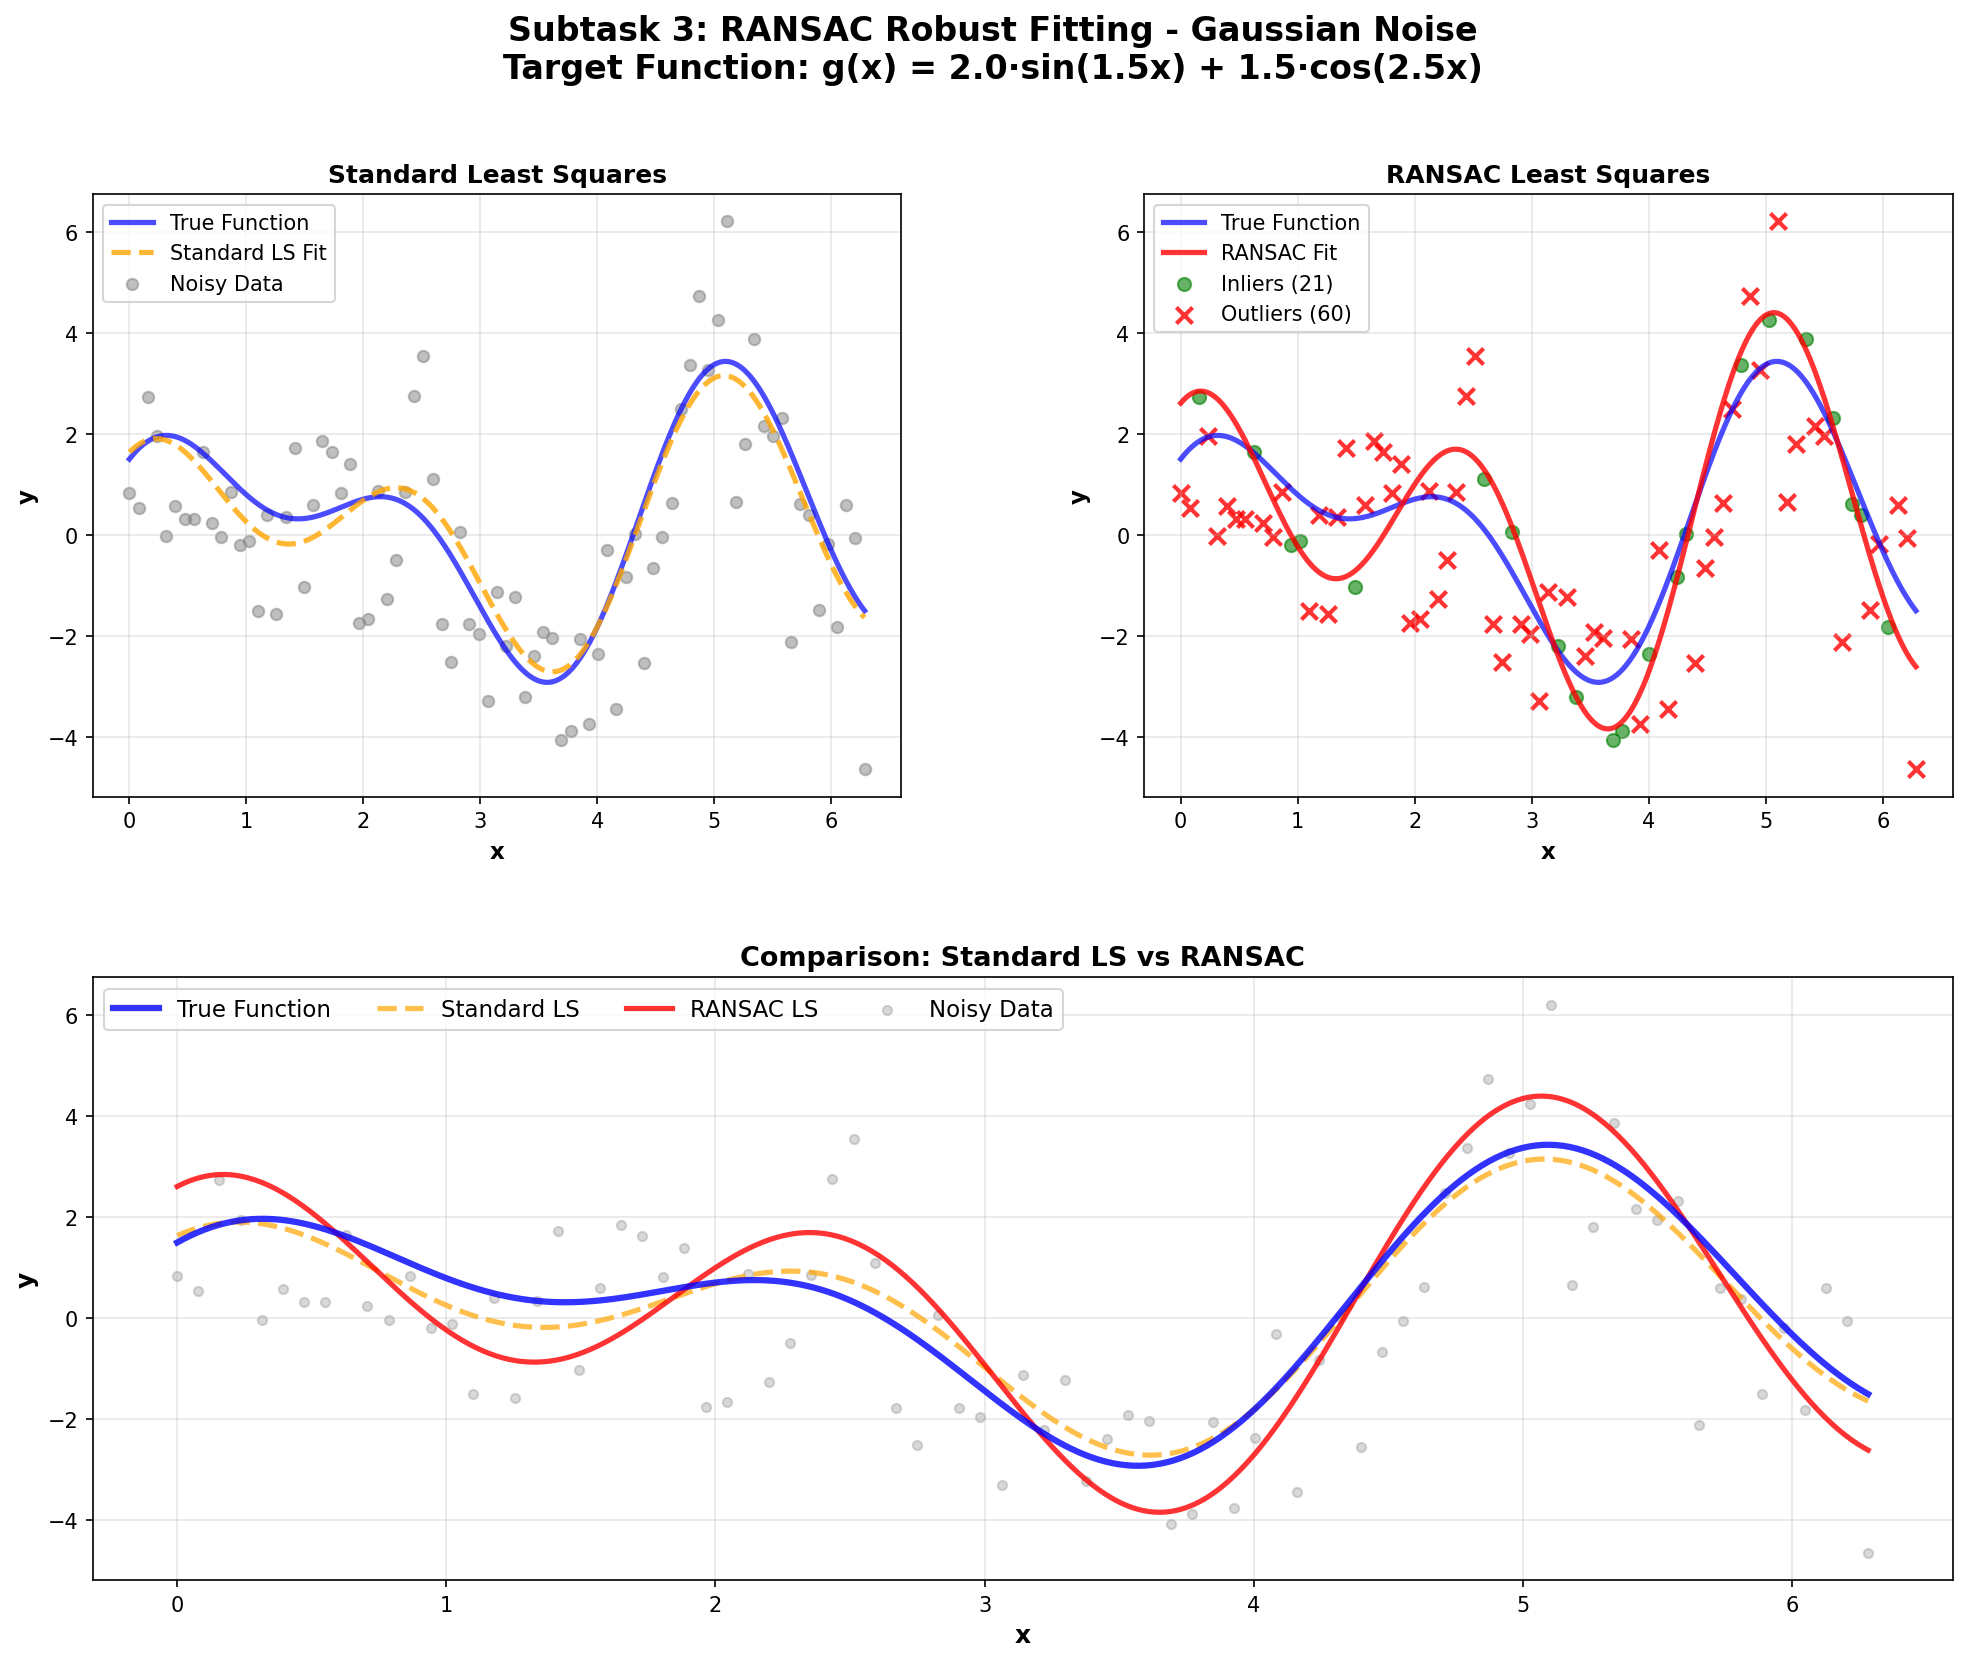
\includegraphics[width=0.95\textwidth]{results/task2/subtask3/comparison_gaussian_noise.png}
\caption{高斯噪声场景:RANSAC vs 标准最小二乘}
\label{fig:task2_subtask3_gaussian}
\end{figure}

图\ref{fig:task2_subtask3_gaussian}展示了高斯噪声场景下的拟合结果。可以看到:
\begin{itemize}
    \item 标准最小二乘法能够有效处理全局分布的高斯噪声
    \item RANSAC错误地将大量正常点判定为离群点(内点率仅26\%)
    \item 这导致RANSAC拟合曲线严重偏离真实函数
\end{itemize}

\begin{figure}[H]
\centering
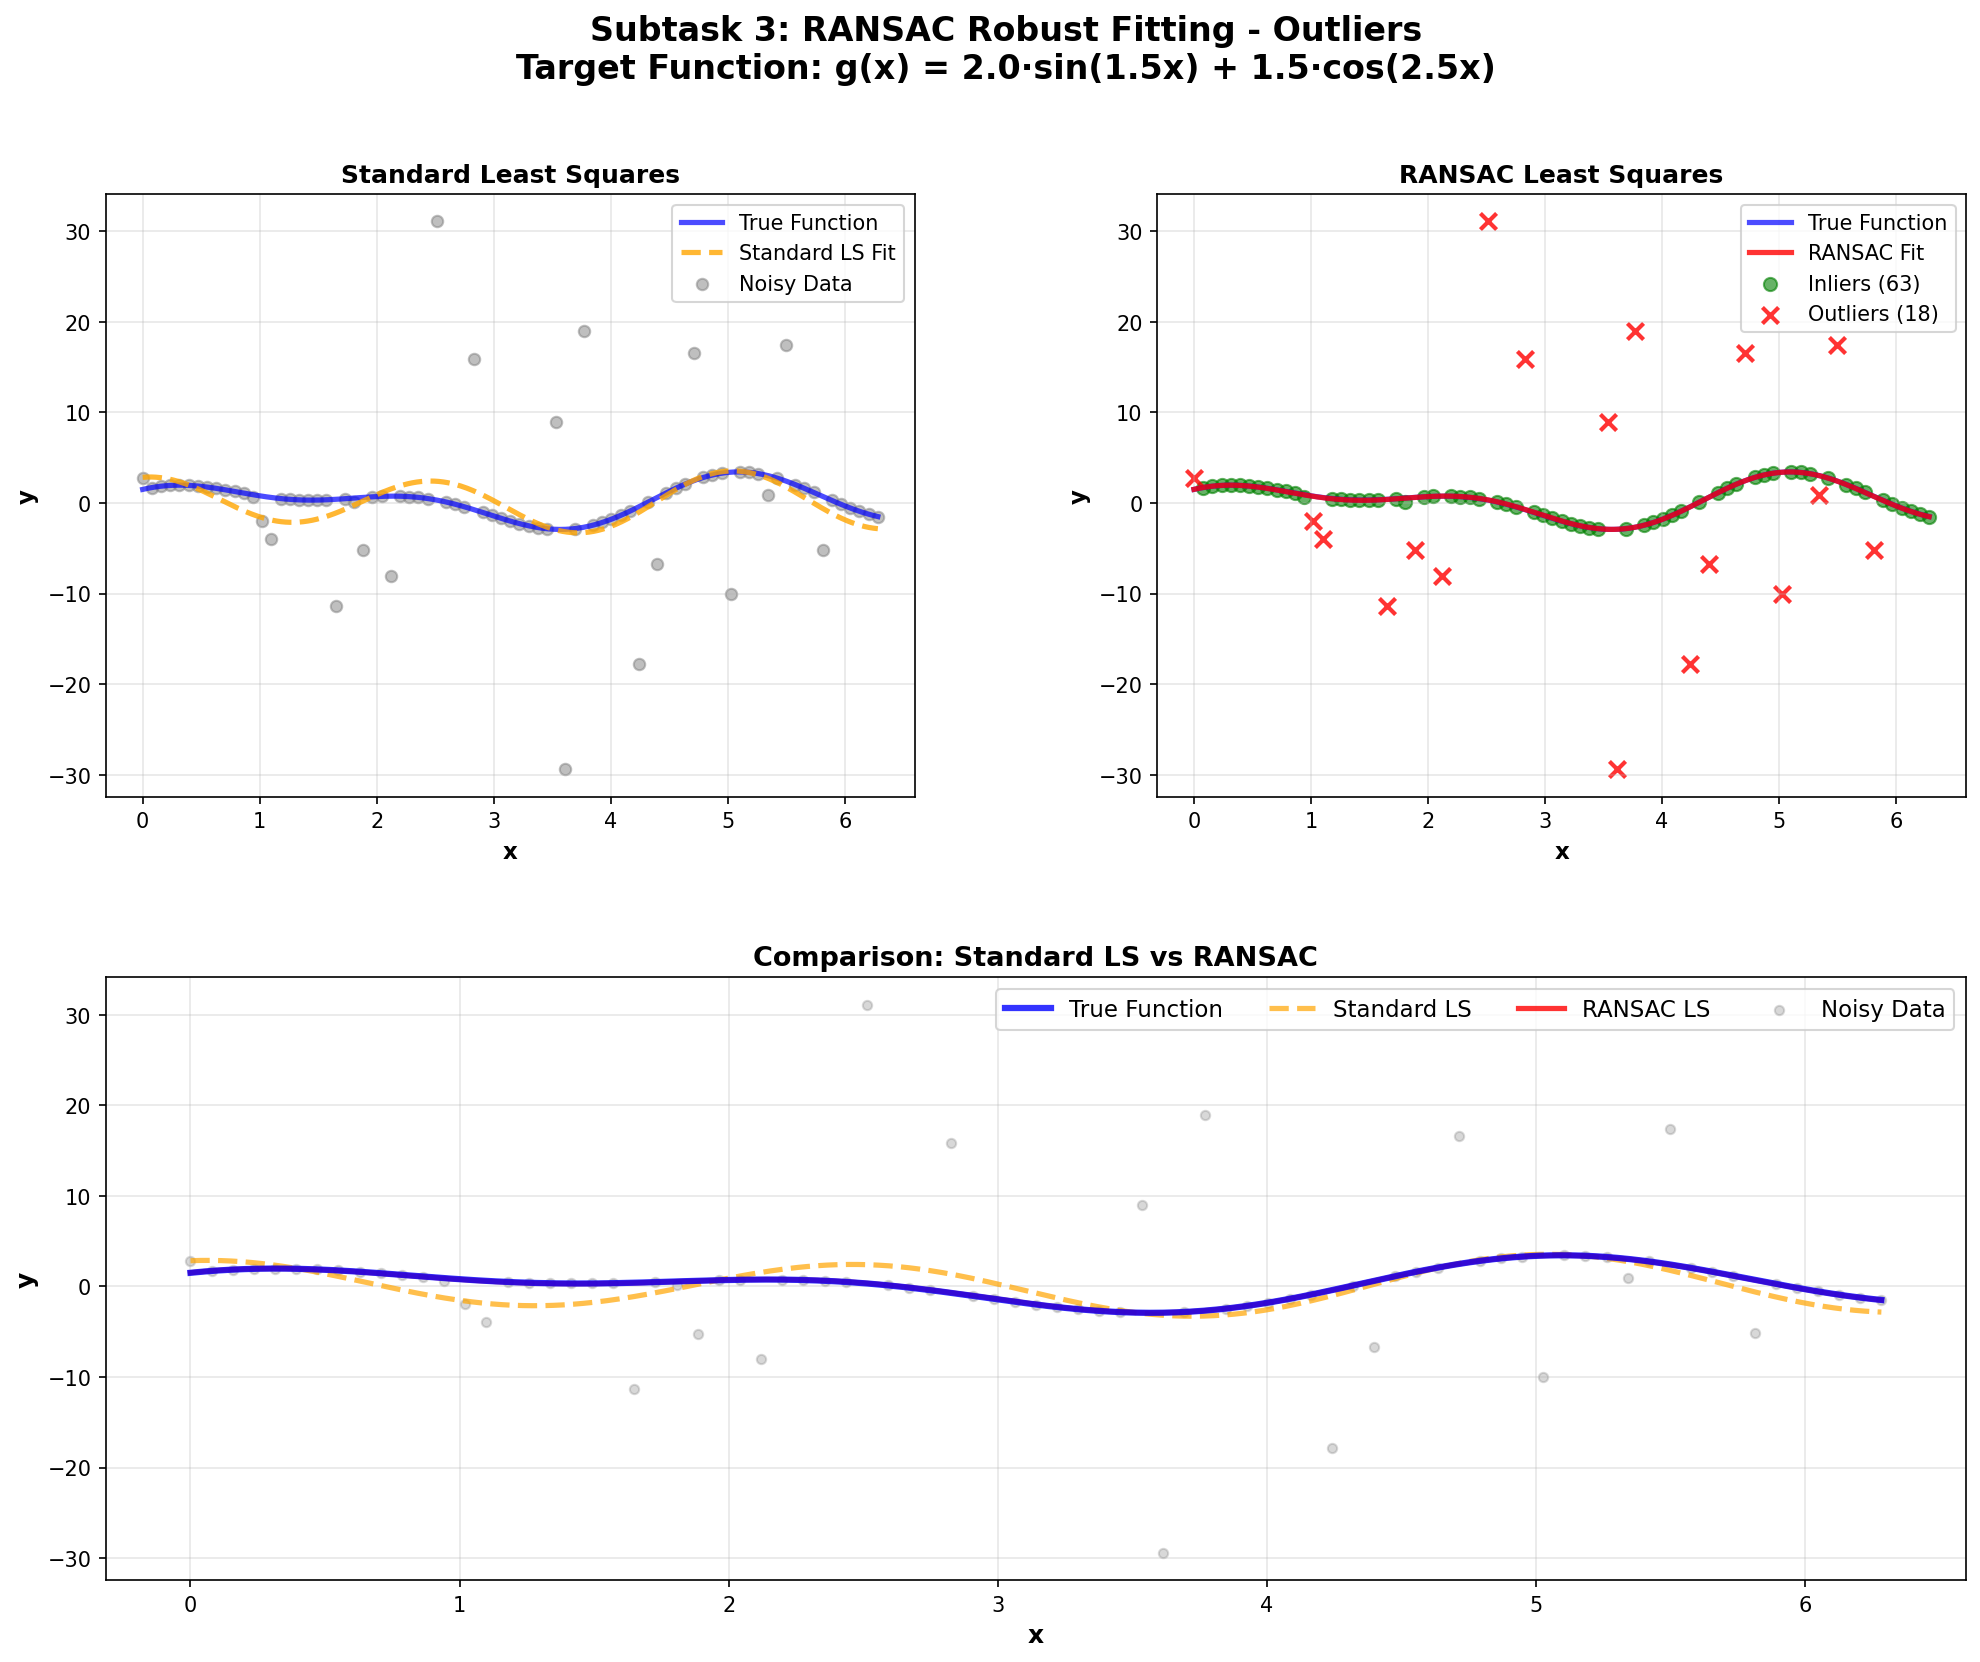
\includegraphics[width=0.95\textwidth]{results/task2/subtask3/comparison_outliers.png}
\caption{离群点场景:RANSAC vs 标准最小二乘}
\label{fig:task2_subtask3_outliers}
\end{figure}

图\ref{fig:task2_subtask3_outliers}展示了离群点场景下的拟合结果。可以看到:
\begin{itemize}
    \item RANSAC成功识别并排除了25\%的离群点(内点率77.78\%)
    \item RANSAC拟合曲线几乎完美重合于真实函数
    \item 标准最小二乘法受离群点影响,拟合曲线明显偏离
\end{itemize}

\begin{figure}[H]
\centering
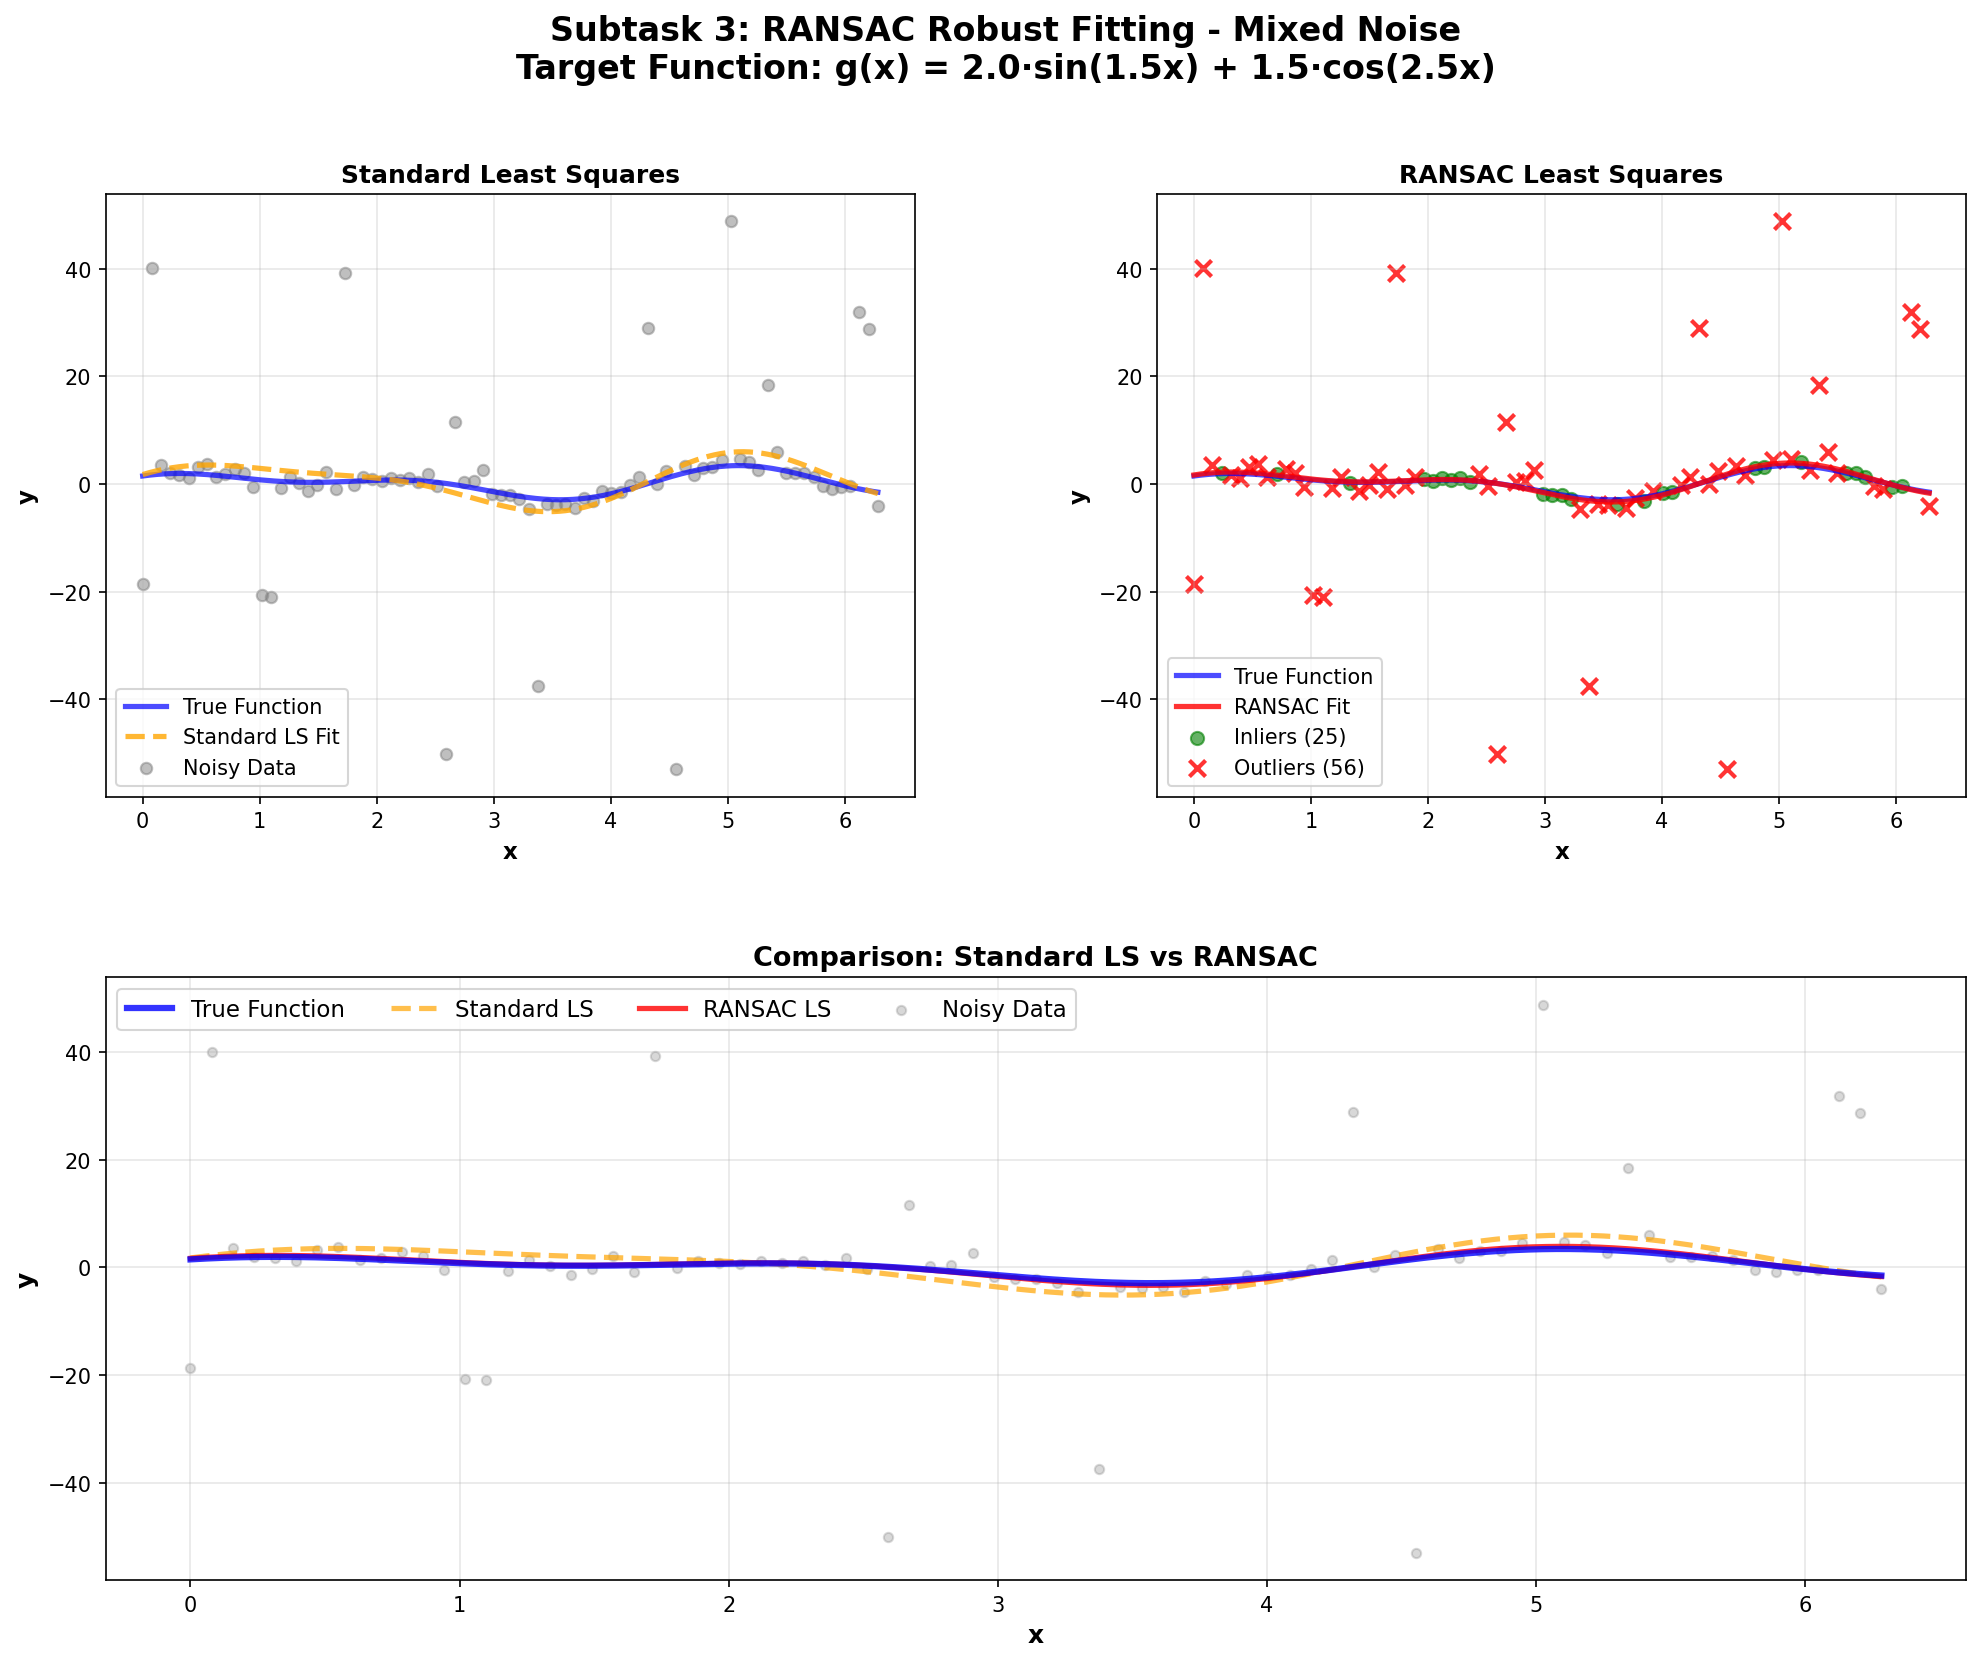
\includegraphics[width=0.95\textwidth]{results/task2/subtask3/comparison_mixed_noise.png}
\caption{混合噪声场景:RANSAC vs 标准最小二乘}
\label{fig:task2_subtask3_mixed}
\end{figure}

图\ref{fig:task2_subtask3_mixed}展示了混合噪声场景下的拟合结果。可以看到:
\begin{itemize}
    \item RANSAC在高斯噪声和离群点的混合场景下仍保持较好性能
    \item 虽然内点率降低至30.86\%,但拟合质量仍优于标准方法
    \item 这验证了RANSAC在复杂噪声环境下的鲁棒性
\end{itemize}

\subsubsection{结果分析}

\begin{tcolorbox}[enhanced,colback=green!5!white,colframe=green!50!black,title=RANSAC性能评估]

\textbf{优势场景}:
\begin{itemize}
    \item \textbf{离群点}:RANSAC表现卓越,RMSE从1.30降至0.01(99\%改善)
    \item \textbf{混合噪声}:显著优于标准方法(85\%改善)
    \item 内点比例:离群点场景77.78\%,混合噪声30.86\%
\end{itemize}

\textbf{劣势场景}:
\begin{itemize}
    \item \textbf{高斯噪声}:RANSAC反而更差(-151\%)
    \item 原因:高斯噪声影响所有点,RANSAC误判许多点为外点(内点仅26\%)
\end{itemize}

\textbf{结论}:RANSAC适合处理少量离群点,不适合全局噪声。

\end{tcolorbox}

\subsection{算法复杂度总结}

\begin{table}[H]
\centering
\caption{各算法的时间和空间复杂度}
\label{tab:complexity}
\begin{tabular}{@{}L{4cm}C{2.5cm}C{2.5cm}@{}}
\toprule
\textbf{算法} & \textbf{时间复杂度} & \textbf{空间复杂度} \\
\midrule
牛顿插值 & $O(n^2)$ & $O(n)$ \\
最小二乘(直接法) & $O(mn^2 + n^3)$ & $O(n^2)$ \\
分段多项式拟合 & $O(m \cdot k \cdot d^3)$ & $O(d^2)$ \\
RANSAC & $O(K \cdot mn^2)$ & $O(m + n^2)$ \\
\bottomrule
\end{tabular}
\end{table}

其中:$n$为基函数数量,$m$为数据点数量,$k$为分段数,$d$为多项式次数,$K$为RANSAC迭代次数。
\newpage
\section{核心算法实现}

本节展示实验中实现的关键算法代码。所有代码均为手工实现,不依赖第三方数值计算库(除勒让德零点外)。

\subsection{采样策略实现}

\subsubsection{切比雪夫节点生成}

\begin{lstlisting}[language=Python,caption={切比雪夫节点生成算法}]
def chebyshev_nodes(n, a=-1, b=1):
    """
    生成切比雪夫节点
    x_k = cos((2k-1)*pi/(2n)), k=1,2,...,n
    """
    import math
    nodes = []
    for k in range(1, n + 1):
        # 标准区间[-1,1]上的切比雪夫零点
        x_standard = math.cos((2*k - 1) * math.pi / (2*n))
        # 映射到[a,b]区间
        x_mapped = 0.5 * (a + b) + 0.5 * (b - a) * x_standard
        nodes.append(x_mapped)
    nodes.sort()
    return nodes
\end{lstlisting}

\subsection{插值算法实现}

\subsubsection{牛顿差商计算}

\begin{lstlisting}[language=Python,caption={牛顿差商表计算}]
def newton_divided_difference(x_points, y_points):
    """
    计算牛顿差商表
    返回插值多项式系数: [f[x_0], f[x_0,x_1], ..., f[x_0,...,x_n]]
    """
    n = len(x_points)
    divided_diff = [[0.0] * n for _ in range(n)]
    
    # 第0列: f[x_i] = y_i
    for i in range(n):
        divided_diff[i][0] = y_points[i]
    
    # 递推计算高阶差商
    for j in range(1, n):
        for i in range(n - j):
            numerator = divided_diff[i+1][j-1] - divided_diff[i][j-1]
            denominator = x_points[i+j] - x_points[i]
            divided_diff[i][j] = numerator / denominator
    
    return [divided_diff[0][j] for j in range(n)]
\end{lstlisting}

\subsubsection{牛顿插值多项式求值}

\begin{lstlisting}[language=Python,caption={牛顿插值求值(霍纳法则)}]
def evaluate_interpolation_batch(x_sample, coeffs, x_eval):
    """
    批量计算牛顿插值多项式值
    N(x) = c_0 + c_1(x-x_0) + c_2(x-x_0)(x-x_1) + ...
    """
    results = []
    for x in x_eval:
        y = coeffs[0]
        prod = 1.0
        for i in range(1, len(coeffs)):
            prod *= (x - x_sample[i-1])
            y += coeffs[i] * prod
        results.append(y)
    return results
\end{lstlisting}

\subsection{矩阵运算实现}

\subsubsection{矩阵类核心方法}

\begin{lstlisting}[language=Python,caption={矩阵类的关键方法}]
class Matrix:
    def transpose(self):
        """矩阵转置"""
        transposed_data = [[self.data[j][i] for j in range(self.rows)]
                          for i in range(self.cols)]
        return Matrix(transposed_data)
    
    def multiply(self, other):
        """矩阵乘法 A * B"""
        if self.cols != other.rows:
            raise ValueError("矩阵维度不匹配")
        
        result_data = [[0.0 for _ in range(other.cols)]
                      for _ in range(self.rows)]
        
        for i in range(self.rows):
            for j in range(other.cols):
                for k in range(self.cols):
                    result_data[i][j] += self.data[i][k] * other.data[k][j]
        
        return Matrix(result_data)
\end{lstlisting}

\subsubsection{高斯消元法求解线性方程组}

\begin{lstlisting}[language=Python,caption={高斯消元法(列主元选取)}]
def solve_linear_system(self, b):
    """
    求解线性方程组 Ax = b
    使用列主元Gauss消元法,提高数值稳定性
    """
    n = self.rows
    augmented = [self.data[i][:] + [b[i]] for i in range(n)]
    
    # 前向消元(列主元)
    for col in range(n):
        # 选择列主元
        max_row = max(range(col, n), 
                     key=lambda i: abs(augmented[i][col]))
        augmented[col], augmented[max_row] = \
            augmented[max_row], augmented[col]
        
        # 消元
        for row in range(col + 1, n):
            factor = augmented[row][col] / augmented[col][col]
            for j in range(col, n + 1):
                augmented[row][j] -= factor * augmented[col][j]
    
    # 回代求解
    x = [0.0] * n
    for i in range(n - 1, -1, -1):
        x[i] = augmented[i][n]
        for j in range(i + 1, n):
            x[i] -= augmented[i][j] * x[j]
        x[i] /= augmented[i][i]
    
    return x
\end{lstlisting}

\subsection{最小二乘拟合实现}

\subsubsection{最小二乘法核心算法}

\begin{lstlisting}[language=Python,caption={最小二乘拟合核心实现}]
def least_squares_fit(x_data, y_data, basis_functions):
    """
    最小二乘拟合
    求解法方程: (A^T A)c = A^T y
    """
    n_data = len(x_data)
    n_basis = len(basis_functions)
    
    # 构造设计矩阵 A[i][j] = phi_j(x_i)
    A_data = []
    for i in range(n_data):
        row = [basis_func(x_data[i]) for basis_func in basis_functions]
        A_data.append(row)
    
    A = Matrix(A_data)
    
    # 求解法方程
    AT = A.transpose()
    ATA = AT.multiply(A)
    ATy = AT.multiply(Matrix.from_vector(y_data))
    
    coefficients = ATA.solve_linear_system(ATy)
    
    return coefficients
\end{lstlisting}

\subsubsection{分段多项式拟合}

\begin{lstlisting}[language=Python,caption={分段多项式拟合算法}]
def piecewise_fit(x_data, y_data, num_segments, degree):
    """
    分段多项式拟合
    将区间等分为num_segments段,每段用degree次多项式拟合
    """
    # 创建区间
    x_min, x_max = min(x_data), max(x_data)
    intervals = create_intervals(x_min, x_max, num_segments)
    
    segment_coeffs = []
    segment_ranges = []
    
    for seg_idx, (a, b) in enumerate(intervals):
        # 选择当前段的数据点
        is_last = (seg_idx == len(intervals) - 1)
        indices = [i for i, x in enumerate(x_data)
                  if (a <= x < b) or (is_last and x == b)]
        
        if len(indices) < degree + 1:
            actual_degree = max(0, len(indices) - 1)
        else:
            actual_degree = degree
        
        x_segment = [x_data[i] for i in indices]
        y_segment = [y_data[i] for i in indices]
        
        # 多项式拟合
        basis_funcs = polynomial_basis(actual_degree)
        coeffs = least_squares_fit(x_segment, y_segment, basis_funcs)
        
        segment_coeffs.append((coeffs, actual_degree))
        segment_ranges.append((a, b))
    
    return segment_coeffs, segment_ranges
\end{lstlisting}

\subsection{RANSAC鲁棒拟合}

\begin{lstlisting}[language=Python,caption={RANSAC算法实现}]
def ransac_fit(x_data, y_data, basis_functions, 
               max_iterations=1000, threshold=0.5, min_samples=5):
    """
    RANSAC鲁棒拟合算法
    能够排除离群点的影响
    """
    import random
    
    best_model = None
    best_inliers = []
    max_inlier_count = 0
    
    for iteration in range(max_iterations):
        # 随机选择最小样本集
        if len(x_data) < min_samples:
            min_samples = len(x_data)
        
        sample_indices = random.sample(range(len(x_data)), min_samples)
        x_sample = [x_data[i] for i in sample_indices]
        y_sample = [y_data[i] for i in sample_indices]
        
        # 拟合模型
        try:
            coeffs = least_squares_fit(x_sample, y_sample, basis_functions)
        except:
            continue
        
        # 计算所有点的残差
        residuals = compute_residuals(x_data, y_data, 
                                      coeffs, basis_functions)
        
        # 统计内点
        inliers = [i for i, res in enumerate(residuals) 
                  if abs(res) < threshold]
        
        # 更新最佳模型
        if len(inliers) > max_inlier_count:
            max_inlier_count = len(inliers)
            best_inliers = inliers
            best_model = coeffs
    
    # 使用所有内点重新拟合
    if best_inliers:
        x_inliers = [x_data[i] for i in best_inliers]
        y_inliers = [y_data[i] for i in best_inliers]
        final_model = least_squares_fit(x_inliers, y_inliers, 
                                       basis_functions)
        return final_model, best_inliers
    
    return best_model, best_inliers
\end{lstlisting}

\end{document}
